\documentclass[twoside]{book}

% Packages required by doxygen
\usepackage{fixltx2e}
\usepackage{calc}
\usepackage{doxygen}
\usepackage[export]{adjustbox} % also loads graphicx
\usepackage{graphicx}
\usepackage[utf8]{inputenc}
\usepackage{makeidx}
\usepackage{multicol}
\usepackage{multirow}
\PassOptionsToPackage{warn}{textcomp}
\usepackage{textcomp}
\usepackage[nointegrals]{wasysym}
\usepackage[table]{xcolor}

% Font selection
\usepackage[T1]{fontenc}
\usepackage[scaled=.90]{helvet}
\usepackage{courier}
\usepackage{amssymb}
\usepackage{sectsty}
\renewcommand{\familydefault}{\sfdefault}
\allsectionsfont{%
  \fontseries{bc}\selectfont%
  \color{darkgray}%
}
\renewcommand{\DoxyLabelFont}{%
  \fontseries{bc}\selectfont%
  \color{darkgray}%
}
\newcommand{\+}{\discretionary{\mbox{\scriptsize$\hookleftarrow$}}{}{}}

% Page & text layout
\usepackage{geometry}
\geometry{%
  a4paper,%
  top=2.5cm,%
  bottom=2.5cm,%
  left=2.5cm,%
  right=2.5cm%
}
\tolerance=750
\hfuzz=15pt
\hbadness=750
\setlength{\emergencystretch}{15pt}
\setlength{\parindent}{0cm}
\setlength{\parskip}{3ex plus 2ex minus 2ex}
\makeatletter
\renewcommand{\paragraph}{%
  \@startsection{paragraph}{4}{0ex}{-1.0ex}{1.0ex}{%
    \normalfont\normalsize\bfseries\SS@parafont%
  }%
}
\renewcommand{\subparagraph}{%
  \@startsection{subparagraph}{5}{0ex}{-1.0ex}{1.0ex}{%
    \normalfont\normalsize\bfseries\SS@subparafont%
  }%
}
\makeatother

% Headers & footers
\usepackage{fancyhdr}
\pagestyle{fancyplain}
\fancyhead[LE]{\fancyplain{}{\bfseries\thepage}}
\fancyhead[CE]{\fancyplain{}{}}
\fancyhead[RE]{\fancyplain{}{\bfseries\leftmark}}
\fancyhead[LO]{\fancyplain{}{\bfseries\rightmark}}
\fancyhead[CO]{\fancyplain{}{}}
\fancyhead[RO]{\fancyplain{}{\bfseries\thepage}}
\fancyfoot[LE]{\fancyplain{}{}}
\fancyfoot[CE]{\fancyplain{}{}}
\fancyfoot[RE]{\fancyplain{}{\bfseries\scriptsize Generated by Doxygen }}
\fancyfoot[LO]{\fancyplain{}{\bfseries\scriptsize Generated by Doxygen }}
\fancyfoot[CO]{\fancyplain{}{}}
\fancyfoot[RO]{\fancyplain{}{}}
\renewcommand{\footrulewidth}{0.4pt}
\renewcommand{\chaptermark}[1]{%
  \markboth{#1}{}%
}
\renewcommand{\sectionmark}[1]{%
  \markright{\thesection\ #1}%
}

% Indices & bibliography
\usepackage{natbib}
\usepackage[titles]{tocloft}
\setcounter{tocdepth}{3}
\setcounter{secnumdepth}{5}
\makeindex

% Hyperlinks (required, but should be loaded last)
\usepackage{ifpdf}
\ifpdf
  \usepackage[pdftex,pagebackref=true]{hyperref}
\else
  \usepackage[ps2pdf,pagebackref=true]{hyperref}
\fi
\hypersetup{%
  colorlinks=true,%
  linkcolor=blue,%
  citecolor=blue,%
  unicode%
}

% Custom commands
\newcommand{\clearemptydoublepage}{%
  \newpage{\pagestyle{empty}\cleardoublepage}%
}

\usepackage{caption}
\captionsetup{labelsep=space,justification=centering,font={bf},singlelinecheck=off,skip=4pt,position=top}

%===== C O N T E N T S =====

\begin{document}

% Titlepage & ToC
\hypersetup{pageanchor=false,
             bookmarksnumbered=true,
             pdfencoding=unicode
            }
\pagenumbering{alph}
\begin{titlepage}
\vspace*{7cm}
\begin{center}%
{\Large Rata-\/2020 }\\
\vspace*{1cm}
{\large Generated by Doxygen 1.8.13}\\
\end{center}
\end{titlepage}
\clearemptydoublepage
\pagenumbering{roman}
\tableofcontents
\clearemptydoublepage
\pagenumbering{arabic}
\hypersetup{pageanchor=true}

%--- Begin generated contents ---
\chapter{Class Index}
\section{Class List}
Here are the classes, structs, unions and interfaces with brief descriptions\+:\begin{DoxyCompactList}
\item\contentsline{section}{\hyperlink{struct_s_t_r_u___c_s_v___c_o_u_n_t}{S\+T\+R\+U\+\_\+\+C\+S\+V\+\_\+\+C\+O\+U\+NT} }{\pageref{struct_s_t_r_u___c_s_v___c_o_u_n_t}}{}
\item\contentsline{section}{\hyperlink{struct_s_t_r_u___d_e_m_o}{S\+T\+R\+U\+\_\+\+D\+E\+MO} }{\pageref{struct_s_t_r_u___d_e_m_o}}{}
\end{DoxyCompactList}

\chapter{File Index}
\section{File List}
Here is a list of all files with brief descriptions\+:\begin{DoxyCompactList}
\item\contentsline{section}{\hyperlink{sd__app_8c}{sd\+\_\+app.\+c} \\*Sd\+\_\+card functions for application }{\pageref{sd__app_8c}}{}
\item\contentsline{section}{\hyperlink{sd__app_8h}{sd\+\_\+app.\+h} }{\pageref{sd__app_8h}}{}
\item\contentsline{section}{\hyperlink{sd__manage__lib_8c}{sd\+\_\+manage\+\_\+lib.\+c} \\*Contain functions to manage read and write sd card action }{\pageref{sd__manage__lib_8c}}{}
\item\contentsline{section}{\hyperlink{sd__manage__lib_8h}{sd\+\_\+manage\+\_\+lib.\+h} }{\pageref{sd__manage__lib_8h}}{}
\end{DoxyCompactList}

\chapter{Class Documentation}
\hypertarget{struct_s_t_r_u___c_s_v___c_o_u_n_t}{}\section{S\+T\+R\+U\+\_\+\+C\+S\+V\+\_\+\+C\+O\+U\+NT Struct Reference}
\label{struct_s_t_r_u___c_s_v___c_o_u_n_t}\index{S\+T\+R\+U\+\_\+\+C\+S\+V\+\_\+\+C\+O\+U\+NT@{S\+T\+R\+U\+\_\+\+C\+S\+V\+\_\+\+C\+O\+U\+NT}}


{\ttfamily \#include $<$sd\+\_\+manage\+\_\+lib.\+h$>$}

\subsection*{Public Attributes}
\begin{DoxyCompactItemize}
\item 
uint16\+\_\+t \hyperlink{struct_s_t_r_u___c_s_v___c_o_u_n_t_a4af4f2506d9d9de6cc194b64a077940d}{u16\+\_\+fields}
\item 
uint16\+\_\+t \hyperlink{struct_s_t_r_u___c_s_v___c_o_u_n_t_af557890ea741e79fd5d4a6b7593a379c}{u16\+\_\+rows}
\end{DoxyCompactItemize}


\subsection{Detailed Description}
Struct contain content of csv file 

\subsection{Member Data Documentation}
\mbox{\Hypertarget{struct_s_t_r_u___c_s_v___c_o_u_n_t_a4af4f2506d9d9de6cc194b64a077940d}\label{struct_s_t_r_u___c_s_v___c_o_u_n_t_a4af4f2506d9d9de6cc194b64a077940d}} 
\index{S\+T\+R\+U\+\_\+\+C\+S\+V\+\_\+\+C\+O\+U\+NT@{S\+T\+R\+U\+\_\+\+C\+S\+V\+\_\+\+C\+O\+U\+NT}!u16\+\_\+fields@{u16\+\_\+fields}}
\index{u16\+\_\+fields@{u16\+\_\+fields}!S\+T\+R\+U\+\_\+\+C\+S\+V\+\_\+\+C\+O\+U\+NT@{S\+T\+R\+U\+\_\+\+C\+S\+V\+\_\+\+C\+O\+U\+NT}}
\subsubsection{\texorpdfstring{u16\+\_\+fields}{u16\_fields}}
{\footnotesize\ttfamily uint16\+\_\+t S\+T\+R\+U\+\_\+\+C\+S\+V\+\_\+\+C\+O\+U\+N\+T\+::u16\+\_\+fields}

\mbox{\Hypertarget{struct_s_t_r_u___c_s_v___c_o_u_n_t_af557890ea741e79fd5d4a6b7593a379c}\label{struct_s_t_r_u___c_s_v___c_o_u_n_t_af557890ea741e79fd5d4a6b7593a379c}} 
\index{S\+T\+R\+U\+\_\+\+C\+S\+V\+\_\+\+C\+O\+U\+NT@{S\+T\+R\+U\+\_\+\+C\+S\+V\+\_\+\+C\+O\+U\+NT}!u16\+\_\+rows@{u16\+\_\+rows}}
\index{u16\+\_\+rows@{u16\+\_\+rows}!S\+T\+R\+U\+\_\+\+C\+S\+V\+\_\+\+C\+O\+U\+NT@{S\+T\+R\+U\+\_\+\+C\+S\+V\+\_\+\+C\+O\+U\+NT}}
\subsubsection{\texorpdfstring{u16\+\_\+rows}{u16\_rows}}
{\footnotesize\ttfamily uint16\+\_\+t S\+T\+R\+U\+\_\+\+C\+S\+V\+\_\+\+C\+O\+U\+N\+T\+::u16\+\_\+rows}



The documentation for this struct was generated from the following file\+:\begin{DoxyCompactItemize}
\item 
\hyperlink{sd__manage__lib_8h}{sd\+\_\+manage\+\_\+lib.\+h}\end{DoxyCompactItemize}

\hypertarget{struct_s_t_r_u___d_e_m_o}{}\section{S\+T\+R\+U\+\_\+\+D\+E\+MO Struct Reference}
\label{struct_s_t_r_u___d_e_m_o}\index{S\+T\+R\+U\+\_\+\+D\+E\+MO@{S\+T\+R\+U\+\_\+\+D\+E\+MO}}


{\ttfamily \#include $<$header\+\_\+template.\+h$>$}

\subsection*{Public Attributes}
\begin{DoxyCompactItemize}
\item 
uint8\+\_\+t \hyperlink{struct_s_t_r_u___d_e_m_o_a79ae9788d6fe743339242fc3369a482e}{u8\+\_\+demo\+\_\+value}
\end{DoxyCompactItemize}


\subsection{Detailed Description}
A description of the struct. 

\subsection{Member Data Documentation}
\mbox{\Hypertarget{struct_s_t_r_u___d_e_m_o_a79ae9788d6fe743339242fc3369a482e}\label{struct_s_t_r_u___d_e_m_o_a79ae9788d6fe743339242fc3369a482e}} 
\index{S\+T\+R\+U\+\_\+\+D\+E\+MO@{S\+T\+R\+U\+\_\+\+D\+E\+MO}!u8\+\_\+demo\+\_\+value@{u8\+\_\+demo\+\_\+value}}
\index{u8\+\_\+demo\+\_\+value@{u8\+\_\+demo\+\_\+value}!S\+T\+R\+U\+\_\+\+D\+E\+MO@{S\+T\+R\+U\+\_\+\+D\+E\+MO}}
\subsubsection{\texorpdfstring{u8\+\_\+demo\+\_\+value}{u8\_demo\_value}}
{\footnotesize\ttfamily uint8\+\_\+t S\+T\+R\+U\+\_\+\+D\+E\+M\+O\+::u8\+\_\+demo\+\_\+value}

Some documentation for u8\+\_\+demo\+\_\+value 

The documentation for this struct was generated from the following file\+:\begin{DoxyCompactItemize}
\item 
\hyperlink{header__template_8h}{header\+\_\+template.\+h}\end{DoxyCompactItemize}

\chapter{File Documentation}
\hypertarget{sd__app_8c}{}\section{sd\+\_\+app.\+c File Reference}
\label{sd__app_8c}\index{sd\+\_\+app.\+c@{sd\+\_\+app.\+c}}


sd\+\_\+card functions for application  


{\ttfamily \#include $<$stdint.\+h$>$}\newline
{\ttfamily \#include $<$string.\+h$>$}\newline
{\ttfamily \#include \char`\"{}sd\+\_\+manage\+\_\+lib.\+h\char`\"{}}\newline
{\ttfamily \#include \char`\"{}sd\+\_\+app.\+h\char`\"{}}\newline
{\ttfamily \#include \char`\"{}crc32.\+h\char`\"{}}\newline
{\ttfamily \#include \char`\"{}Free\+R\+T\+O\+S.\+h\char`\"{}}\newline
{\ttfamily \#include \char`\"{}task.\+h\char`\"{}}\newline
Include dependency graph for sd\+\_\+app.\+c\+:
\nopagebreak
\begin{figure}[H]
\begin{center}
\leavevmode
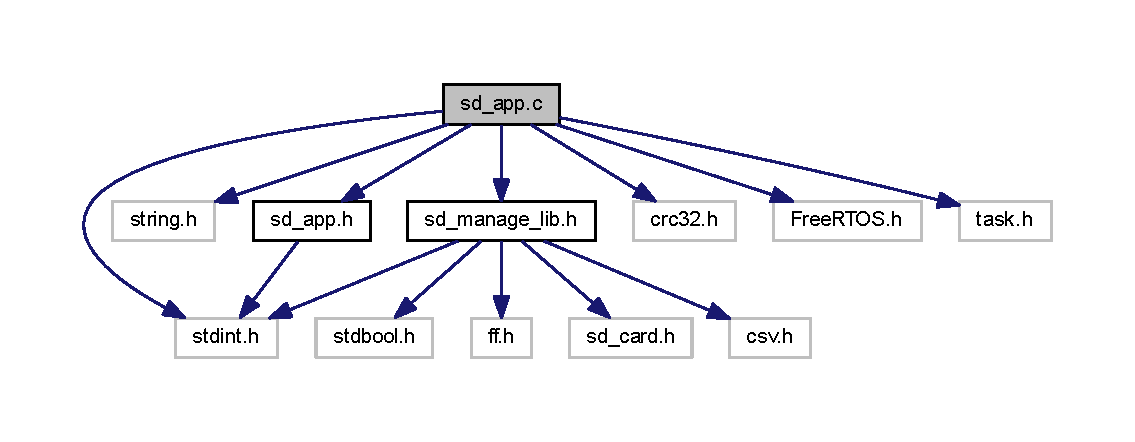
\includegraphics[width=350pt]{sd__app_8c__incl}
\end{center}
\end{figure}
\subsection*{Macros}
\begin{DoxyCompactItemize}
\item 
\#define \hyperlink{sd__app_8c_a30c74414c5f2ce1866c6e0e0879748cb}{C\+S\+V\+\_\+\+C\+O\+M\+M\+E\+N\+T\+\_\+\+L\+I\+N\+E\+\_\+\+F\+I\+R\+S\+T\+\_\+\+C\+H\+AR}~\textquotesingle{}\#\textquotesingle{}
\item 
\#define \hyperlink{sd__app_8c_a69631d1f497ccd6c4b4a4d570f4e8a7a}{C\+S\+V\+\_\+\+Q\+U\+O\+T\+E\+\_\+\+C\+H\+AR}~\textquotesingle{}\char`\"{}\textquotesingle{}
\item 
\#define \hyperlink{sd__app_8c_ae0716c24fb751c324a63db353bf04f07}{C\+S\+V\+\_\+\+B\+U\+F\+F\+E\+R\+\_\+\+L\+E\+N\+G\+T\+H\+\_\+\+R\+E\+A\+D\+\_\+\+L\+I\+NE}~300
\end{DoxyCompactItemize}
\subsection*{Functions}
\begin{DoxyCompactItemize}
\item 
int8\+\_\+t \hyperlink{sd__app_8c_a275b018ff39b6472d64bbb1eeabe6ea0}{i8\+\_\+handle\+\_\+csv\+\_\+file\+\_\+callback} (char $\ast$txtname, void($\ast$cb1)(void $\ast$, size\+\_\+t, void $\ast$), void($\ast$cb2)(int c, void $\ast$), void $\ast$c)
\begin{DoxyCompactList}\small\item\em process a csv file \end{DoxyCompactList}\item 
int8\+\_\+t \hyperlink{sd__app_8c_ad196e69ccf05c1d47e43749901bc50ba}{i8\+\_\+sdcard\+\_\+save\+\_\+schedule\+\_\+version} (char $\ast$version)
\begin{DoxyCompactList}\small\item\em save version of schedule file \end{DoxyCompactList}\item 
int8\+\_\+t \hyperlink{sd__app_8c_a95ae7469ae17b7cd923e6ebe8b1598b2}{i8\+\_\+sdcard\+\_\+get\+\_\+schedule\+\_\+version} (char $\ast$version)
\begin{DoxyCompactList}\small\item\em get version of schedule file \end{DoxyCompactList}\item 
int8\+\_\+t \hyperlink{sd__app_8c_a1df205e28a74e07c47c6accd37e3b5a6}{i8\+\_\+sdcard\+\_\+save\+\_\+mainflow} (uint8\+\_\+t u8\+\_\+location\+\_\+id, uint32\+\_\+t u32\+\_\+main\+\_\+flow)
\begin{DoxyCompactList}\small\item\em save flow rate of main flow meter for a given location \end{DoxyCompactList}\item 
int8\+\_\+t \hyperlink{sd__app_8c_ab63ec937ddc9cab6582404b12c6a7681}{i8\+\_\+sdcard\+\_\+get\+\_\+mainflow} (uint8\+\_\+t u8\+\_\+location\+\_\+id, uint32\+\_\+t $\ast$pu32\+\_\+main\+\_\+flow)
\begin{DoxyCompactList}\small\item\em get flow rate of main flow meter for a given location \end{DoxyCompactList}\item 
int8\+\_\+t \hyperlink{sd__app_8c_ae6f9db7bf77ba864120025515b8b00ed}{i8\+\_\+sdcard\+\_\+save\+\_\+channels\+\_\+flow} (uint8\+\_\+t u8\+\_\+location\+\_\+id, uint16\+\_\+t $\ast$pu16\+\_\+channels\+\_\+flow)
\begin{DoxyCompactList}\small\item\em save flow rate of 5 fertilizer channels for a given location \end{DoxyCompactList}\item 
int8\+\_\+t \hyperlink{sd__app_8c_abaa7c724857f50bc2de767a171581a5d}{i8\+\_\+sdcard\+\_\+get\+\_\+channels\+\_\+flow} (uint8\+\_\+t u8\+\_\+location\+\_\+id, uint16\+\_\+t $\ast$pu16\+\_\+channels\+\_\+flow)
\begin{DoxyCompactList}\small\item\em get flow rate of 5 fertilizer channels flow meter for a given location \end{DoxyCompactList}\end{DoxyCompactItemize}


\subsection{Detailed Description}
sd\+\_\+card functions for application 

\begin{DoxyAuthor}{Author}
Danh Pham 
\end{DoxyAuthor}
\begin{DoxyDate}{Date}
11 Nov 2020 
\end{DoxyDate}
\begin{DoxyVersion}{Version}
\+: 2.\+0.\+0 
\end{DoxyVersion}


\subsection{Macro Definition Documentation}
\mbox{\Hypertarget{sd__app_8c_ae0716c24fb751c324a63db353bf04f07}\label{sd__app_8c_ae0716c24fb751c324a63db353bf04f07}} 
\index{sd\+\_\+app.\+c@{sd\+\_\+app.\+c}!C\+S\+V\+\_\+\+B\+U\+F\+F\+E\+R\+\_\+\+L\+E\+N\+G\+T\+H\+\_\+\+R\+E\+A\+D\+\_\+\+L\+I\+NE@{C\+S\+V\+\_\+\+B\+U\+F\+F\+E\+R\+\_\+\+L\+E\+N\+G\+T\+H\+\_\+\+R\+E\+A\+D\+\_\+\+L\+I\+NE}}
\index{C\+S\+V\+\_\+\+B\+U\+F\+F\+E\+R\+\_\+\+L\+E\+N\+G\+T\+H\+\_\+\+R\+E\+A\+D\+\_\+\+L\+I\+NE@{C\+S\+V\+\_\+\+B\+U\+F\+F\+E\+R\+\_\+\+L\+E\+N\+G\+T\+H\+\_\+\+R\+E\+A\+D\+\_\+\+L\+I\+NE}!sd\+\_\+app.\+c@{sd\+\_\+app.\+c}}
\subsubsection{\texorpdfstring{C\+S\+V\+\_\+\+B\+U\+F\+F\+E\+R\+\_\+\+L\+E\+N\+G\+T\+H\+\_\+\+R\+E\+A\+D\+\_\+\+L\+I\+NE}{CSV\_BUFFER\_LENGTH\_READ\_LINE}}
{\footnotesize\ttfamily \#define C\+S\+V\+\_\+\+B\+U\+F\+F\+E\+R\+\_\+\+L\+E\+N\+G\+T\+H\+\_\+\+R\+E\+A\+D\+\_\+\+L\+I\+NE~300}

Maximum lenght of one csv line \mbox{\Hypertarget{sd__app_8c_a30c74414c5f2ce1866c6e0e0879748cb}\label{sd__app_8c_a30c74414c5f2ce1866c6e0e0879748cb}} 
\index{sd\+\_\+app.\+c@{sd\+\_\+app.\+c}!C\+S\+V\+\_\+\+C\+O\+M\+M\+E\+N\+T\+\_\+\+L\+I\+N\+E\+\_\+\+F\+I\+R\+S\+T\+\_\+\+C\+H\+AR@{C\+S\+V\+\_\+\+C\+O\+M\+M\+E\+N\+T\+\_\+\+L\+I\+N\+E\+\_\+\+F\+I\+R\+S\+T\+\_\+\+C\+H\+AR}}
\index{C\+S\+V\+\_\+\+C\+O\+M\+M\+E\+N\+T\+\_\+\+L\+I\+N\+E\+\_\+\+F\+I\+R\+S\+T\+\_\+\+C\+H\+AR@{C\+S\+V\+\_\+\+C\+O\+M\+M\+E\+N\+T\+\_\+\+L\+I\+N\+E\+\_\+\+F\+I\+R\+S\+T\+\_\+\+C\+H\+AR}!sd\+\_\+app.\+c@{sd\+\_\+app.\+c}}
\subsubsection{\texorpdfstring{C\+S\+V\+\_\+\+C\+O\+M\+M\+E\+N\+T\+\_\+\+L\+I\+N\+E\+\_\+\+F\+I\+R\+S\+T\+\_\+\+C\+H\+AR}{CSV\_COMMENT\_LINE\_FIRST\_CHAR}}
{\footnotesize\ttfamily \#define C\+S\+V\+\_\+\+C\+O\+M\+M\+E\+N\+T\+\_\+\+L\+I\+N\+E\+\_\+\+F\+I\+R\+S\+T\+\_\+\+C\+H\+AR~\textquotesingle{}\#\textquotesingle{}}

\mbox{\Hypertarget{sd__app_8c_a69631d1f497ccd6c4b4a4d570f4e8a7a}\label{sd__app_8c_a69631d1f497ccd6c4b4a4d570f4e8a7a}} 
\index{sd\+\_\+app.\+c@{sd\+\_\+app.\+c}!C\+S\+V\+\_\+\+Q\+U\+O\+T\+E\+\_\+\+C\+H\+AR@{C\+S\+V\+\_\+\+Q\+U\+O\+T\+E\+\_\+\+C\+H\+AR}}
\index{C\+S\+V\+\_\+\+Q\+U\+O\+T\+E\+\_\+\+C\+H\+AR@{C\+S\+V\+\_\+\+Q\+U\+O\+T\+E\+\_\+\+C\+H\+AR}!sd\+\_\+app.\+c@{sd\+\_\+app.\+c}}
\subsubsection{\texorpdfstring{C\+S\+V\+\_\+\+Q\+U\+O\+T\+E\+\_\+\+C\+H\+AR}{CSV\_QUOTE\_CHAR}}
{\footnotesize\ttfamily \#define C\+S\+V\+\_\+\+Q\+U\+O\+T\+E\+\_\+\+C\+H\+AR~\textquotesingle{}\char`\"{}\textquotesingle{}}



\subsection{Function Documentation}
\mbox{\Hypertarget{sd__app_8c_a275b018ff39b6472d64bbb1eeabe6ea0}\label{sd__app_8c_a275b018ff39b6472d64bbb1eeabe6ea0}} 
\index{sd\+\_\+app.\+c@{sd\+\_\+app.\+c}!i8\+\_\+handle\+\_\+csv\+\_\+file\+\_\+callback@{i8\+\_\+handle\+\_\+csv\+\_\+file\+\_\+callback}}
\index{i8\+\_\+handle\+\_\+csv\+\_\+file\+\_\+callback@{i8\+\_\+handle\+\_\+csv\+\_\+file\+\_\+callback}!sd\+\_\+app.\+c@{sd\+\_\+app.\+c}}
\subsubsection{\texorpdfstring{i8\+\_\+handle\+\_\+csv\+\_\+file\+\_\+callback()}{i8\_handle\_csv\_file\_callback()}}
{\footnotesize\ttfamily i8\+\_\+handle\+\_\+csv\+\_\+file\+\_\+callback (\begin{DoxyParamCaption}\item[{char $\ast$}]{txtname,  }\item[{void($\ast$)(void $\ast$, size\+\_\+t, void $\ast$)}]{cb1,  }\item[{void($\ast$)(int c, void $\ast$)}]{cb2,  }\item[{void $\ast$}]{c }\end{DoxyParamCaption})}



process a csv file 

Variables declare

Private functions prototype

Public functions


\begin{DoxyParams}[1]{Parameters}
\mbox{\tt in}  & {\em txtname} & name of file \\
\hline
\mbox{\tt in}  & {\em cb1} & function to parse row of file \\
\hline
\mbox{\tt in}  & {\em cb2} & function to parse feild in row \\
\hline
\mbox{\tt in}  & {\em c} & buffer of file \\
\hline
\end{DoxyParams}
\begin{DoxyReturn}{Returns}
0\+: read success -\/1\+: can not init file -\/2\+: file is not exist -\/3\+: fail to parse file -\/4\+: C\+RC error 
\end{DoxyReturn}
Here is the call graph for this function\+:
\nopagebreak
\begin{figure}[H]
\begin{center}
\leavevmode
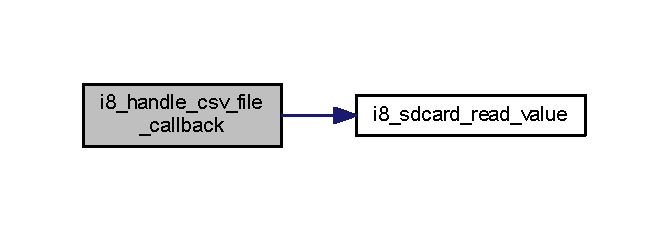
\includegraphics[width=321pt]{sd__app_8c_a275b018ff39b6472d64bbb1eeabe6ea0_cgraph}
\end{center}
\end{figure}
\mbox{\Hypertarget{sd__app_8c_abaa7c724857f50bc2de767a171581a5d}\label{sd__app_8c_abaa7c724857f50bc2de767a171581a5d}} 
\index{sd\+\_\+app.\+c@{sd\+\_\+app.\+c}!i8\+\_\+sdcard\+\_\+get\+\_\+channels\+\_\+flow@{i8\+\_\+sdcard\+\_\+get\+\_\+channels\+\_\+flow}}
\index{i8\+\_\+sdcard\+\_\+get\+\_\+channels\+\_\+flow@{i8\+\_\+sdcard\+\_\+get\+\_\+channels\+\_\+flow}!sd\+\_\+app.\+c@{sd\+\_\+app.\+c}}
\subsubsection{\texorpdfstring{i8\+\_\+sdcard\+\_\+get\+\_\+channels\+\_\+flow()}{i8\_sdcard\_get\_channels\_flow()}}
{\footnotesize\ttfamily i8\+\_\+sdcard\+\_\+get\+\_\+channels\+\_\+flow (\begin{DoxyParamCaption}\item[{uint8\+\_\+t}]{u8\+\_\+location\+\_\+id,  }\item[{uint16\+\_\+t $\ast$}]{pu16\+\_\+channels\+\_\+flow }\end{DoxyParamCaption})}



get flow rate of 5 fertilizer channels flow meter for a given location 


\begin{DoxyParams}[1]{Parameters}
\mbox{\tt in}  & {\em u8\+\_\+location\+\_\+id} & Id of given location \\
\hline
\mbox{\tt out}  & {\em pu16\+\_\+channels\+\_\+flow} & flow rate \\
\hline
\end{DoxyParams}
\begin{DoxyReturn}{Returns}
0\+: read success -\/1\+: file is not exist -\/2\+: can not read 
\end{DoxyReturn}
Here is the call graph for this function\+:
\nopagebreak
\begin{figure}[H]
\begin{center}
\leavevmode
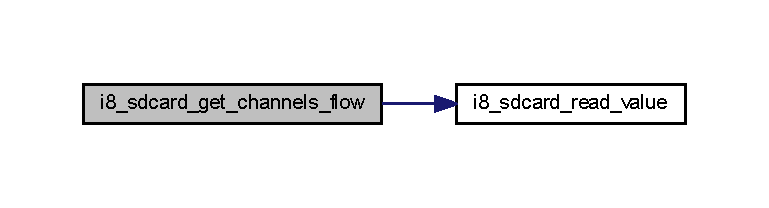
\includegraphics[width=350pt]{sd__app_8c_abaa7c724857f50bc2de767a171581a5d_cgraph}
\end{center}
\end{figure}
\mbox{\Hypertarget{sd__app_8c_ab63ec937ddc9cab6582404b12c6a7681}\label{sd__app_8c_ab63ec937ddc9cab6582404b12c6a7681}} 
\index{sd\+\_\+app.\+c@{sd\+\_\+app.\+c}!i8\+\_\+sdcard\+\_\+get\+\_\+mainflow@{i8\+\_\+sdcard\+\_\+get\+\_\+mainflow}}
\index{i8\+\_\+sdcard\+\_\+get\+\_\+mainflow@{i8\+\_\+sdcard\+\_\+get\+\_\+mainflow}!sd\+\_\+app.\+c@{sd\+\_\+app.\+c}}
\subsubsection{\texorpdfstring{i8\+\_\+sdcard\+\_\+get\+\_\+mainflow()}{i8\_sdcard\_get\_mainflow()}}
{\footnotesize\ttfamily i8\+\_\+sdcard\+\_\+get\+\_\+mainflow (\begin{DoxyParamCaption}\item[{uint8\+\_\+t}]{u8\+\_\+location\+\_\+id,  }\item[{uint32\+\_\+t $\ast$}]{pu32\+\_\+main\+\_\+flow }\end{DoxyParamCaption})}



get flow rate of main flow meter for a given location 


\begin{DoxyParams}[1]{Parameters}
\mbox{\tt in}  & {\em u8\+\_\+location\+\_\+id} & Id of given location \\
\hline
\mbox{\tt out}  & {\em pu32\+\_\+main\+\_\+flow} & flow rate (real value $\ast$ 10) Ex\+: the real value is 10.\+5m3/h =$>$ save value\+: 105 \\
\hline
\end{DoxyParams}
\begin{DoxyReturn}{Returns}
0\+: read success -\/1\+: file is not exist -\/2\+: can not read 
\end{DoxyReturn}
Here is the call graph for this function\+:
\nopagebreak
\begin{figure}[H]
\begin{center}
\leavevmode
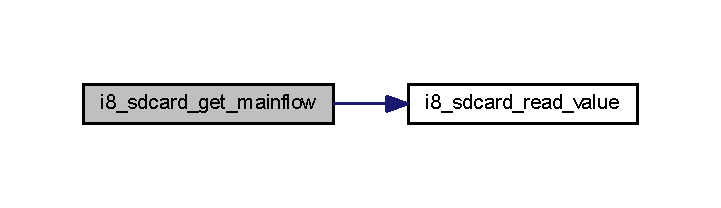
\includegraphics[width=346pt]{sd__app_8c_ab63ec937ddc9cab6582404b12c6a7681_cgraph}
\end{center}
\end{figure}
\mbox{\Hypertarget{sd__app_8c_a95ae7469ae17b7cd923e6ebe8b1598b2}\label{sd__app_8c_a95ae7469ae17b7cd923e6ebe8b1598b2}} 
\index{sd\+\_\+app.\+c@{sd\+\_\+app.\+c}!i8\+\_\+sdcard\+\_\+get\+\_\+schedule\+\_\+version@{i8\+\_\+sdcard\+\_\+get\+\_\+schedule\+\_\+version}}
\index{i8\+\_\+sdcard\+\_\+get\+\_\+schedule\+\_\+version@{i8\+\_\+sdcard\+\_\+get\+\_\+schedule\+\_\+version}!sd\+\_\+app.\+c@{sd\+\_\+app.\+c}}
\subsubsection{\texorpdfstring{i8\+\_\+sdcard\+\_\+get\+\_\+schedule\+\_\+version()}{i8\_sdcard\_get\_schedule\_version()}}
{\footnotesize\ttfamily i8\+\_\+sdcard\+\_\+get\+\_\+schedule\+\_\+version (\begin{DoxyParamCaption}\item[{char $\ast$}]{version }\end{DoxyParamCaption})}



get version of schedule file 


\begin{DoxyParams}[1]{Parameters}
\mbox{\tt out}  & {\em version} & version of schedule file \\
\hline
\end{DoxyParams}
\begin{DoxyReturn}{Returns}
0\+: read success -\/1\+: file is not exist -\/2\+: can not write 
\end{DoxyReturn}
Here is the call graph for this function\+:
\nopagebreak
\begin{figure}[H]
\begin{center}
\leavevmode
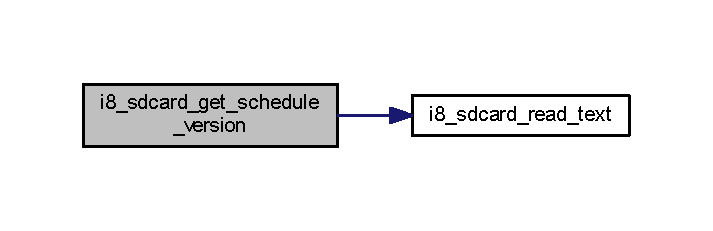
\includegraphics[width=342pt]{sd__app_8c_a95ae7469ae17b7cd923e6ebe8b1598b2_cgraph}
\end{center}
\end{figure}
\mbox{\Hypertarget{sd__app_8c_ae6f9db7bf77ba864120025515b8b00ed}\label{sd__app_8c_ae6f9db7bf77ba864120025515b8b00ed}} 
\index{sd\+\_\+app.\+c@{sd\+\_\+app.\+c}!i8\+\_\+sdcard\+\_\+save\+\_\+channels\+\_\+flow@{i8\+\_\+sdcard\+\_\+save\+\_\+channels\+\_\+flow}}
\index{i8\+\_\+sdcard\+\_\+save\+\_\+channels\+\_\+flow@{i8\+\_\+sdcard\+\_\+save\+\_\+channels\+\_\+flow}!sd\+\_\+app.\+c@{sd\+\_\+app.\+c}}
\subsubsection{\texorpdfstring{i8\+\_\+sdcard\+\_\+save\+\_\+channels\+\_\+flow()}{i8\_sdcard\_save\_channels\_flow()}}
{\footnotesize\ttfamily i8\+\_\+sdcard\+\_\+save\+\_\+channels\+\_\+flow (\begin{DoxyParamCaption}\item[{uint8\+\_\+t}]{u8\+\_\+location\+\_\+id,  }\item[{uint16\+\_\+t $\ast$}]{pu16\+\_\+channels\+\_\+flow }\end{DoxyParamCaption})}



save flow rate of 5 fertilizer channels for a given location 


\begin{DoxyParams}[1]{Parameters}
\mbox{\tt in}  & {\em Id} & of given location \\
\hline
\mbox{\tt in}  & {\em pu16\+\_\+channels\+\_\+flow} & flow rate \\
\hline
\end{DoxyParams}
\begin{DoxyReturn}{Returns}
0\+: read success -\/1\+: file is not exist -\/2\+: can not write 
\end{DoxyReturn}
Here is the call graph for this function\+:
\nopagebreak
\begin{figure}[H]
\begin{center}
\leavevmode
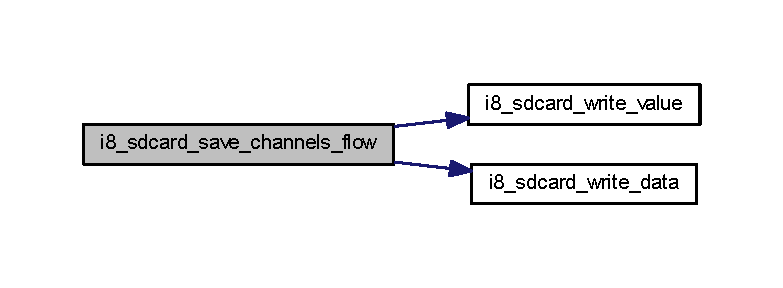
\includegraphics[width=350pt]{sd__app_8c_ae6f9db7bf77ba864120025515b8b00ed_cgraph}
\end{center}
\end{figure}
\mbox{\Hypertarget{sd__app_8c_a1df205e28a74e07c47c6accd37e3b5a6}\label{sd__app_8c_a1df205e28a74e07c47c6accd37e3b5a6}} 
\index{sd\+\_\+app.\+c@{sd\+\_\+app.\+c}!i8\+\_\+sdcard\+\_\+save\+\_\+mainflow@{i8\+\_\+sdcard\+\_\+save\+\_\+mainflow}}
\index{i8\+\_\+sdcard\+\_\+save\+\_\+mainflow@{i8\+\_\+sdcard\+\_\+save\+\_\+mainflow}!sd\+\_\+app.\+c@{sd\+\_\+app.\+c}}
\subsubsection{\texorpdfstring{i8\+\_\+sdcard\+\_\+save\+\_\+mainflow()}{i8\_sdcard\_save\_mainflow()}}
{\footnotesize\ttfamily i8\+\_\+sdcard\+\_\+save\+\_\+mainflow (\begin{DoxyParamCaption}\item[{uint8\+\_\+t}]{u8\+\_\+location\+\_\+id,  }\item[{uint32\+\_\+t}]{u32\+\_\+main\+\_\+flow }\end{DoxyParamCaption})}



save flow rate of main flow meter for a given location 


\begin{DoxyParams}[1]{Parameters}
\mbox{\tt in}  & {\em u8\+\_\+location\+\_\+id} & Id of given location \\
\hline
\mbox{\tt in}  & {\em u32\+\_\+main\+\_\+flow} & flow rate (real value $\ast$ 10) Ex\+: the real value is 10.\+5m3/h =$>$ save value\+: 105 \\
\hline
\end{DoxyParams}
\begin{DoxyReturn}{Returns}
0\+: read success -\/1\+: file is not exist -\/2\+: can not write 
\end{DoxyReturn}
Here is the call graph for this function\+:
\nopagebreak
\begin{figure}[H]
\begin{center}
\leavevmode
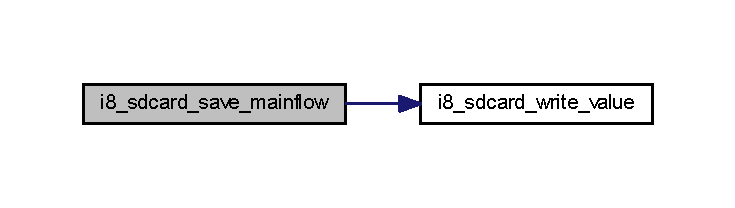
\includegraphics[width=350pt]{sd__app_8c_a1df205e28a74e07c47c6accd37e3b5a6_cgraph}
\end{center}
\end{figure}
\mbox{\Hypertarget{sd__app_8c_ad196e69ccf05c1d47e43749901bc50ba}\label{sd__app_8c_ad196e69ccf05c1d47e43749901bc50ba}} 
\index{sd\+\_\+app.\+c@{sd\+\_\+app.\+c}!i8\+\_\+sdcard\+\_\+save\+\_\+schedule\+\_\+version@{i8\+\_\+sdcard\+\_\+save\+\_\+schedule\+\_\+version}}
\index{i8\+\_\+sdcard\+\_\+save\+\_\+schedule\+\_\+version@{i8\+\_\+sdcard\+\_\+save\+\_\+schedule\+\_\+version}!sd\+\_\+app.\+c@{sd\+\_\+app.\+c}}
\subsubsection{\texorpdfstring{i8\+\_\+sdcard\+\_\+save\+\_\+schedule\+\_\+version()}{i8\_sdcard\_save\_schedule\_version()}}
{\footnotesize\ttfamily i8\+\_\+sdcard\+\_\+save\+\_\+schedule\+\_\+version (\begin{DoxyParamCaption}\item[{char $\ast$}]{version }\end{DoxyParamCaption})}



save version of schedule file 


\begin{DoxyParams}[1]{Parameters}
\mbox{\tt in}  & {\em version} & version of schedule file \\
\hline
\end{DoxyParams}
\begin{DoxyReturn}{Returns}
0\+: read success -\/2\+: can not write 
\end{DoxyReturn}
Here is the call graph for this function\+:
\nopagebreak
\begin{figure}[H]
\begin{center}
\leavevmode
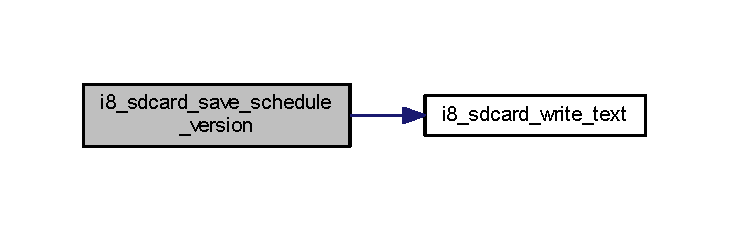
\includegraphics[width=350pt]{sd__app_8c_ad196e69ccf05c1d47e43749901bc50ba_cgraph}
\end{center}
\end{figure}

\hypertarget{sd__app_8h}{}\section{sd\+\_\+app.\+h File Reference}
\label{sd__app_8h}\index{sd\+\_\+app.\+h@{sd\+\_\+app.\+h}}
{\ttfamily \#include $<$stdint.\+h$>$}\newline
Include dependency graph for sd\+\_\+app.\+h\+:
\nopagebreak
\begin{figure}[H]
\begin{center}
\leavevmode
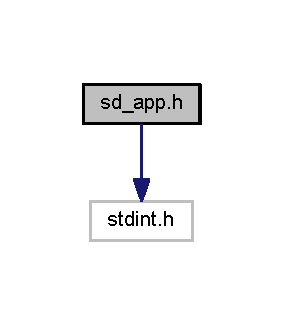
\includegraphics[width=136pt]{sd__app_8h__incl}
\end{center}
\end{figure}
This graph shows which files directly or indirectly include this file\+:
\nopagebreak
\begin{figure}[H]
\begin{center}
\leavevmode
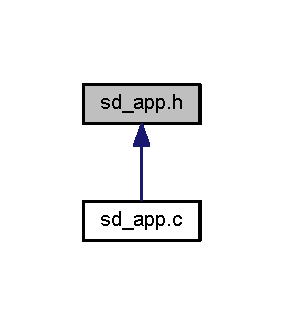
\includegraphics[width=136pt]{sd__app_8h__dep__incl}
\end{center}
\end{figure}
\subsection*{Classes}
\begin{DoxyCompactItemize}
\item 
struct \hyperlink{struct_s_t_r_u___d_e_m_o}{S\+T\+R\+U\+\_\+\+D\+E\+MO}
\end{DoxyCompactItemize}
\subsection*{Macros}
\begin{DoxyCompactItemize}
\item 
\#define \hyperlink{sd__app_8h_ac47979ec2895fc67334287cbab9aeabd}{C\+S\+V\+\_\+\+M\+A\+X\+\_\+\+R\+OW}~(1000)
\item 
\#define \hyperlink{sd__app_8h_abfa4ee0f00c9c824eb1e50e7e3e0cc78}{S\+D\+\_\+\+I\+N\+F\+O\+\_\+\+F\+I\+LE}~\char`\"{}F1.\+B\+IN\char`\"{}
\item 
\#define \hyperlink{sd__app_8h_ad2649e9ec0f3ecf60f81a59521eabf80}{S\+D\+\_\+\+S\+C\+H\+E\+D\+U\+L\+E\+\_\+\+C\+R\+C\+\_\+\+A\+D\+DR}~(0)
\item 
\#define \hyperlink{sd__app_8h_a68b770415676e484139b9decd33c4e82}{S\+D\+\_\+\+S\+C\+H\+E\+D\+U\+L\+E\+\_\+\+V\+E\+R\+\_\+\+A\+D\+DR}~(4)
\item 
\#define \hyperlink{sd__app_8h_a3d75fbda57f5d6a07f35e3f21d59fae5}{S\+D\+\_\+\+F\+L\+O\+W\+\_\+\+F\+I\+LE}~\char`\"{}F2.\+B\+IN\char`\"{}
\item 
\#define \hyperlink{sd__app_8h_a2ede51e63a71d5d1a881abcf7bb8a4ff}{S\+D\+\_\+\+M\+A\+I\+N\+\_\+\+F\+L\+O\+W\+\_\+\+V\+A\+L\+I\+D\+\_\+\+A\+D\+DR}~(0)
\item 
\#define \hyperlink{sd__app_8h_ac4365d89aaaf4416d4c71152545ccbed}{S\+D\+\_\+\+C\+H\+\_\+\+F\+L\+O\+W\+\_\+\+V\+A\+L\+I\+D\+\_\+\+A\+D\+DR}~(4)
\item 
\#define \hyperlink{sd__app_8h_aeae03d33e54e1382bd44c3ba697606c7}{S\+D\+\_\+\+M\+A\+I\+N\+\_\+\+F\+L\+O\+W\+\_\+1\+\_\+\+A\+D\+DR}~(8)
\item 
\#define \hyperlink{sd__app_8h_a1628d131f83cadbdc627cbee7ee5e2de}{S\+D\+\_\+\+C\+H1\+\_\+\+F\+L\+O\+W\+\_\+1\+\_\+\+A\+D\+DR}~(12)
\item 
\#define \hyperlink{sd__app_8h_abc74b1b2ccae5156ec9b8907c2af6e74}{S\+D\+\_\+\+C\+H2\+\_\+\+F\+L\+O\+W\+\_\+1\+\_\+\+A\+D\+DR}~(16)
\item 
\#define \hyperlink{sd__app_8h_a2a81e8429774fe31dda773f519b33ef7}{S\+D\+\_\+\+C\+H3\+\_\+\+F\+L\+O\+W\+\_\+1\+\_\+\+A\+D\+DR}~(20)
\item 
\#define \hyperlink{sd__app_8h_aac741694588b555cddcef8a07479bd12}{S\+D\+\_\+\+C\+H4\+\_\+\+F\+L\+O\+W\+\_\+1\+\_\+\+A\+D\+DR}~(24)
\item 
\#define \hyperlink{sd__app_8h_af05c3fdd088cb417fab4267ef9c25502}{S\+D\+\_\+\+C\+H5\+\_\+\+F\+L\+O\+W\+\_\+1\+\_\+\+A\+D\+DR}~(28)
\end{DoxyCompactItemize}
\subsection*{Enumerations}
\begin{DoxyCompactItemize}
\item 
enum \hyperlink{sd__app_8h_ac927bbf88bd29dd0a1c7715df9fb443c}{E\+\_\+\+D\+E\+MO} \{ \hyperlink{sd__app_8h_ac927bbf88bd29dd0a1c7715df9fb443ca87ef681eef180be8ed49aea2a997406b}{D\+E\+M\+O\+\_\+\+V\+A\+L\+UE} = 0, 
\hyperlink{sd__app_8h_ac927bbf88bd29dd0a1c7715df9fb443ca0d3241fdf12699b594076d73f443f9ba}{D\+E\+M\+O\+\_\+\+V\+A\+L\+U\+E2} = 1
 \}
\end{DoxyCompactItemize}
\subsection*{Functions}
\begin{DoxyCompactItemize}
\item 
int8\+\_\+t \hyperlink{sd__app_8h_a5a7701bf6eb70c9a1ff531d3a7f687ab}{i8\+\_\+handle\+\_\+csv\+\_\+file\+\_\+callback} (char $\ast$txtname, void($\ast$cb1)(void $\ast$, size\+\_\+t, void $\ast$), void($\ast$cb2)(int c, void $\ast$), void $\ast$c)
\begin{DoxyCompactList}\small\item\em process a csv file \end{DoxyCompactList}\item 
int8\+\_\+t \hyperlink{sd__app_8h_a47950b3f5c7eb8ba9316f92109afc47d}{i8\+\_\+sdcard\+\_\+save\+\_\+schedule\+\_\+version} (char $\ast$version)
\begin{DoxyCompactList}\small\item\em save version of schedule file \end{DoxyCompactList}\item 
int8\+\_\+t \hyperlink{sd__app_8h_a33496be7efcfdf272994b216b05eb1f8}{i8\+\_\+sdcard\+\_\+get\+\_\+schedule\+\_\+version} (char $\ast$version)
\begin{DoxyCompactList}\small\item\em get version of schedule file \end{DoxyCompactList}\item 
int8\+\_\+t \hyperlink{sd__app_8h_a046dccab0a39863b7943a5e4aaf26298}{i8\+\_\+sdcard\+\_\+save\+\_\+mainflow} (uint8\+\_\+t u8\+\_\+location\+\_\+id, uint32\+\_\+t u32\+\_\+main\+\_\+flow)
\begin{DoxyCompactList}\small\item\em save flow rate of main flow meter for a given location \end{DoxyCompactList}\item 
int8\+\_\+t \hyperlink{sd__app_8h_a4c963fbbe651d03d8982e219c4166e35}{i8\+\_\+sdcard\+\_\+get\+\_\+mainflow} (uint8\+\_\+t u8\+\_\+location\+\_\+id, uint32\+\_\+t $\ast$pu32\+\_\+main\+\_\+flow)
\begin{DoxyCompactList}\small\item\em get flow rate of main flow meter for a given location \end{DoxyCompactList}\item 
int8\+\_\+t \hyperlink{sd__app_8h_a2d21479adf7864569b3427aadc083579}{i8\+\_\+sdcard\+\_\+save\+\_\+channels\+\_\+flow} (uint8\+\_\+t u8\+\_\+location\+\_\+id, uint16\+\_\+t $\ast$pu16\+\_\+channels\+\_\+flow)
\begin{DoxyCompactList}\small\item\em save flow rate of 5 fertilizer channels for a given location \end{DoxyCompactList}\item 
int8\+\_\+t \hyperlink{sd__app_8h_ac64497358537694b4dd27b4cf9454015}{i8\+\_\+sdcard\+\_\+get\+\_\+channels\+\_\+flow} (uint8\+\_\+t u8\+\_\+location\+\_\+id, uint16\+\_\+t $\ast$pu16\+\_\+channels\+\_\+flow)
\begin{DoxyCompactList}\small\item\em get flow rate of 5 fertilizer channels flow meter for a given location \end{DoxyCompactList}\end{DoxyCompactItemize}


\subsection{Macro Definition Documentation}
\mbox{\Hypertarget{sd__app_8h_ac47979ec2895fc67334287cbab9aeabd}\label{sd__app_8h_ac47979ec2895fc67334287cbab9aeabd}} 
\index{sd\+\_\+app.\+h@{sd\+\_\+app.\+h}!C\+S\+V\+\_\+\+M\+A\+X\+\_\+\+R\+OW@{C\+S\+V\+\_\+\+M\+A\+X\+\_\+\+R\+OW}}
\index{C\+S\+V\+\_\+\+M\+A\+X\+\_\+\+R\+OW@{C\+S\+V\+\_\+\+M\+A\+X\+\_\+\+R\+OW}!sd\+\_\+app.\+h@{sd\+\_\+app.\+h}}
\subsubsection{\texorpdfstring{C\+S\+V\+\_\+\+M\+A\+X\+\_\+\+R\+OW}{CSV\_MAX\_ROW}}
{\footnotesize\ttfamily \#define C\+S\+V\+\_\+\+M\+A\+X\+\_\+\+R\+OW~(1000)}

Maximum rows of csv file \mbox{\Hypertarget{sd__app_8h_a1628d131f83cadbdc627cbee7ee5e2de}\label{sd__app_8h_a1628d131f83cadbdc627cbee7ee5e2de}} 
\index{sd\+\_\+app.\+h@{sd\+\_\+app.\+h}!S\+D\+\_\+\+C\+H1\+\_\+\+F\+L\+O\+W\+\_\+1\+\_\+\+A\+D\+DR@{S\+D\+\_\+\+C\+H1\+\_\+\+F\+L\+O\+W\+\_\+1\+\_\+\+A\+D\+DR}}
\index{S\+D\+\_\+\+C\+H1\+\_\+\+F\+L\+O\+W\+\_\+1\+\_\+\+A\+D\+DR@{S\+D\+\_\+\+C\+H1\+\_\+\+F\+L\+O\+W\+\_\+1\+\_\+\+A\+D\+DR}!sd\+\_\+app.\+h@{sd\+\_\+app.\+h}}
\subsubsection{\texorpdfstring{S\+D\+\_\+\+C\+H1\+\_\+\+F\+L\+O\+W\+\_\+1\+\_\+\+A\+D\+DR}{SD\_CH1\_FLOW\_1\_ADDR}}
{\footnotesize\ttfamily \#define S\+D\+\_\+\+C\+H1\+\_\+\+F\+L\+O\+W\+\_\+1\+\_\+\+A\+D\+DR~(12)}

\mbox{\Hypertarget{sd__app_8h_abc74b1b2ccae5156ec9b8907c2af6e74}\label{sd__app_8h_abc74b1b2ccae5156ec9b8907c2af6e74}} 
\index{sd\+\_\+app.\+h@{sd\+\_\+app.\+h}!S\+D\+\_\+\+C\+H2\+\_\+\+F\+L\+O\+W\+\_\+1\+\_\+\+A\+D\+DR@{S\+D\+\_\+\+C\+H2\+\_\+\+F\+L\+O\+W\+\_\+1\+\_\+\+A\+D\+DR}}
\index{S\+D\+\_\+\+C\+H2\+\_\+\+F\+L\+O\+W\+\_\+1\+\_\+\+A\+D\+DR@{S\+D\+\_\+\+C\+H2\+\_\+\+F\+L\+O\+W\+\_\+1\+\_\+\+A\+D\+DR}!sd\+\_\+app.\+h@{sd\+\_\+app.\+h}}
\subsubsection{\texorpdfstring{S\+D\+\_\+\+C\+H2\+\_\+\+F\+L\+O\+W\+\_\+1\+\_\+\+A\+D\+DR}{SD\_CH2\_FLOW\_1\_ADDR}}
{\footnotesize\ttfamily \#define S\+D\+\_\+\+C\+H2\+\_\+\+F\+L\+O\+W\+\_\+1\+\_\+\+A\+D\+DR~(16)}

\mbox{\Hypertarget{sd__app_8h_a2a81e8429774fe31dda773f519b33ef7}\label{sd__app_8h_a2a81e8429774fe31dda773f519b33ef7}} 
\index{sd\+\_\+app.\+h@{sd\+\_\+app.\+h}!S\+D\+\_\+\+C\+H3\+\_\+\+F\+L\+O\+W\+\_\+1\+\_\+\+A\+D\+DR@{S\+D\+\_\+\+C\+H3\+\_\+\+F\+L\+O\+W\+\_\+1\+\_\+\+A\+D\+DR}}
\index{S\+D\+\_\+\+C\+H3\+\_\+\+F\+L\+O\+W\+\_\+1\+\_\+\+A\+D\+DR@{S\+D\+\_\+\+C\+H3\+\_\+\+F\+L\+O\+W\+\_\+1\+\_\+\+A\+D\+DR}!sd\+\_\+app.\+h@{sd\+\_\+app.\+h}}
\subsubsection{\texorpdfstring{S\+D\+\_\+\+C\+H3\+\_\+\+F\+L\+O\+W\+\_\+1\+\_\+\+A\+D\+DR}{SD\_CH3\_FLOW\_1\_ADDR}}
{\footnotesize\ttfamily \#define S\+D\+\_\+\+C\+H3\+\_\+\+F\+L\+O\+W\+\_\+1\+\_\+\+A\+D\+DR~(20)}

\mbox{\Hypertarget{sd__app_8h_aac741694588b555cddcef8a07479bd12}\label{sd__app_8h_aac741694588b555cddcef8a07479bd12}} 
\index{sd\+\_\+app.\+h@{sd\+\_\+app.\+h}!S\+D\+\_\+\+C\+H4\+\_\+\+F\+L\+O\+W\+\_\+1\+\_\+\+A\+D\+DR@{S\+D\+\_\+\+C\+H4\+\_\+\+F\+L\+O\+W\+\_\+1\+\_\+\+A\+D\+DR}}
\index{S\+D\+\_\+\+C\+H4\+\_\+\+F\+L\+O\+W\+\_\+1\+\_\+\+A\+D\+DR@{S\+D\+\_\+\+C\+H4\+\_\+\+F\+L\+O\+W\+\_\+1\+\_\+\+A\+D\+DR}!sd\+\_\+app.\+h@{sd\+\_\+app.\+h}}
\subsubsection{\texorpdfstring{S\+D\+\_\+\+C\+H4\+\_\+\+F\+L\+O\+W\+\_\+1\+\_\+\+A\+D\+DR}{SD\_CH4\_FLOW\_1\_ADDR}}
{\footnotesize\ttfamily \#define S\+D\+\_\+\+C\+H4\+\_\+\+F\+L\+O\+W\+\_\+1\+\_\+\+A\+D\+DR~(24)}

\mbox{\Hypertarget{sd__app_8h_af05c3fdd088cb417fab4267ef9c25502}\label{sd__app_8h_af05c3fdd088cb417fab4267ef9c25502}} 
\index{sd\+\_\+app.\+h@{sd\+\_\+app.\+h}!S\+D\+\_\+\+C\+H5\+\_\+\+F\+L\+O\+W\+\_\+1\+\_\+\+A\+D\+DR@{S\+D\+\_\+\+C\+H5\+\_\+\+F\+L\+O\+W\+\_\+1\+\_\+\+A\+D\+DR}}
\index{S\+D\+\_\+\+C\+H5\+\_\+\+F\+L\+O\+W\+\_\+1\+\_\+\+A\+D\+DR@{S\+D\+\_\+\+C\+H5\+\_\+\+F\+L\+O\+W\+\_\+1\+\_\+\+A\+D\+DR}!sd\+\_\+app.\+h@{sd\+\_\+app.\+h}}
\subsubsection{\texorpdfstring{S\+D\+\_\+\+C\+H5\+\_\+\+F\+L\+O\+W\+\_\+1\+\_\+\+A\+D\+DR}{SD\_CH5\_FLOW\_1\_ADDR}}
{\footnotesize\ttfamily \#define S\+D\+\_\+\+C\+H5\+\_\+\+F\+L\+O\+W\+\_\+1\+\_\+\+A\+D\+DR~(28)}

\mbox{\Hypertarget{sd__app_8h_ac4365d89aaaf4416d4c71152545ccbed}\label{sd__app_8h_ac4365d89aaaf4416d4c71152545ccbed}} 
\index{sd\+\_\+app.\+h@{sd\+\_\+app.\+h}!S\+D\+\_\+\+C\+H\+\_\+\+F\+L\+O\+W\+\_\+\+V\+A\+L\+I\+D\+\_\+\+A\+D\+DR@{S\+D\+\_\+\+C\+H\+\_\+\+F\+L\+O\+W\+\_\+\+V\+A\+L\+I\+D\+\_\+\+A\+D\+DR}}
\index{S\+D\+\_\+\+C\+H\+\_\+\+F\+L\+O\+W\+\_\+\+V\+A\+L\+I\+D\+\_\+\+A\+D\+DR@{S\+D\+\_\+\+C\+H\+\_\+\+F\+L\+O\+W\+\_\+\+V\+A\+L\+I\+D\+\_\+\+A\+D\+DR}!sd\+\_\+app.\+h@{sd\+\_\+app.\+h}}
\subsubsection{\texorpdfstring{S\+D\+\_\+\+C\+H\+\_\+\+F\+L\+O\+W\+\_\+\+V\+A\+L\+I\+D\+\_\+\+A\+D\+DR}{SD\_CH\_FLOW\_VALID\_ADDR}}
{\footnotesize\ttfamily \#define S\+D\+\_\+\+C\+H\+\_\+\+F\+L\+O\+W\+\_\+\+V\+A\+L\+I\+D\+\_\+\+A\+D\+DR~(4)}

\mbox{\Hypertarget{sd__app_8h_a3d75fbda57f5d6a07f35e3f21d59fae5}\label{sd__app_8h_a3d75fbda57f5d6a07f35e3f21d59fae5}} 
\index{sd\+\_\+app.\+h@{sd\+\_\+app.\+h}!S\+D\+\_\+\+F\+L\+O\+W\+\_\+\+F\+I\+LE@{S\+D\+\_\+\+F\+L\+O\+W\+\_\+\+F\+I\+LE}}
\index{S\+D\+\_\+\+F\+L\+O\+W\+\_\+\+F\+I\+LE@{S\+D\+\_\+\+F\+L\+O\+W\+\_\+\+F\+I\+LE}!sd\+\_\+app.\+h@{sd\+\_\+app.\+h}}
\subsubsection{\texorpdfstring{S\+D\+\_\+\+F\+L\+O\+W\+\_\+\+F\+I\+LE}{SD\_FLOW\_FILE}}
{\footnotesize\ttfamily \#define S\+D\+\_\+\+F\+L\+O\+W\+\_\+\+F\+I\+LE~\char`\"{}F2.\+B\+IN\char`\"{}}

\mbox{\Hypertarget{sd__app_8h_abfa4ee0f00c9c824eb1e50e7e3e0cc78}\label{sd__app_8h_abfa4ee0f00c9c824eb1e50e7e3e0cc78}} 
\index{sd\+\_\+app.\+h@{sd\+\_\+app.\+h}!S\+D\+\_\+\+I\+N\+F\+O\+\_\+\+F\+I\+LE@{S\+D\+\_\+\+I\+N\+F\+O\+\_\+\+F\+I\+LE}}
\index{S\+D\+\_\+\+I\+N\+F\+O\+\_\+\+F\+I\+LE@{S\+D\+\_\+\+I\+N\+F\+O\+\_\+\+F\+I\+LE}!sd\+\_\+app.\+h@{sd\+\_\+app.\+h}}
\subsubsection{\texorpdfstring{S\+D\+\_\+\+I\+N\+F\+O\+\_\+\+F\+I\+LE}{SD\_INFO\_FILE}}
{\footnotesize\ttfamily \#define S\+D\+\_\+\+I\+N\+F\+O\+\_\+\+F\+I\+LE~\char`\"{}F1.\+B\+IN\char`\"{}}

\mbox{\Hypertarget{sd__app_8h_aeae03d33e54e1382bd44c3ba697606c7}\label{sd__app_8h_aeae03d33e54e1382bd44c3ba697606c7}} 
\index{sd\+\_\+app.\+h@{sd\+\_\+app.\+h}!S\+D\+\_\+\+M\+A\+I\+N\+\_\+\+F\+L\+O\+W\+\_\+1\+\_\+\+A\+D\+DR@{S\+D\+\_\+\+M\+A\+I\+N\+\_\+\+F\+L\+O\+W\+\_\+1\+\_\+\+A\+D\+DR}}
\index{S\+D\+\_\+\+M\+A\+I\+N\+\_\+\+F\+L\+O\+W\+\_\+1\+\_\+\+A\+D\+DR@{S\+D\+\_\+\+M\+A\+I\+N\+\_\+\+F\+L\+O\+W\+\_\+1\+\_\+\+A\+D\+DR}!sd\+\_\+app.\+h@{sd\+\_\+app.\+h}}
\subsubsection{\texorpdfstring{S\+D\+\_\+\+M\+A\+I\+N\+\_\+\+F\+L\+O\+W\+\_\+1\+\_\+\+A\+D\+DR}{SD\_MAIN\_FLOW\_1\_ADDR}}
{\footnotesize\ttfamily \#define S\+D\+\_\+\+M\+A\+I\+N\+\_\+\+F\+L\+O\+W\+\_\+1\+\_\+\+A\+D\+DR~(8)}

\mbox{\Hypertarget{sd__app_8h_a2ede51e63a71d5d1a881abcf7bb8a4ff}\label{sd__app_8h_a2ede51e63a71d5d1a881abcf7bb8a4ff}} 
\index{sd\+\_\+app.\+h@{sd\+\_\+app.\+h}!S\+D\+\_\+\+M\+A\+I\+N\+\_\+\+F\+L\+O\+W\+\_\+\+V\+A\+L\+I\+D\+\_\+\+A\+D\+DR@{S\+D\+\_\+\+M\+A\+I\+N\+\_\+\+F\+L\+O\+W\+\_\+\+V\+A\+L\+I\+D\+\_\+\+A\+D\+DR}}
\index{S\+D\+\_\+\+M\+A\+I\+N\+\_\+\+F\+L\+O\+W\+\_\+\+V\+A\+L\+I\+D\+\_\+\+A\+D\+DR@{S\+D\+\_\+\+M\+A\+I\+N\+\_\+\+F\+L\+O\+W\+\_\+\+V\+A\+L\+I\+D\+\_\+\+A\+D\+DR}!sd\+\_\+app.\+h@{sd\+\_\+app.\+h}}
\subsubsection{\texorpdfstring{S\+D\+\_\+\+M\+A\+I\+N\+\_\+\+F\+L\+O\+W\+\_\+\+V\+A\+L\+I\+D\+\_\+\+A\+D\+DR}{SD\_MAIN\_FLOW\_VALID\_ADDR}}
{\footnotesize\ttfamily \#define S\+D\+\_\+\+M\+A\+I\+N\+\_\+\+F\+L\+O\+W\+\_\+\+V\+A\+L\+I\+D\+\_\+\+A\+D\+DR~(0)}

\mbox{\Hypertarget{sd__app_8h_ad2649e9ec0f3ecf60f81a59521eabf80}\label{sd__app_8h_ad2649e9ec0f3ecf60f81a59521eabf80}} 
\index{sd\+\_\+app.\+h@{sd\+\_\+app.\+h}!S\+D\+\_\+\+S\+C\+H\+E\+D\+U\+L\+E\+\_\+\+C\+R\+C\+\_\+\+A\+D\+DR@{S\+D\+\_\+\+S\+C\+H\+E\+D\+U\+L\+E\+\_\+\+C\+R\+C\+\_\+\+A\+D\+DR}}
\index{S\+D\+\_\+\+S\+C\+H\+E\+D\+U\+L\+E\+\_\+\+C\+R\+C\+\_\+\+A\+D\+DR@{S\+D\+\_\+\+S\+C\+H\+E\+D\+U\+L\+E\+\_\+\+C\+R\+C\+\_\+\+A\+D\+DR}!sd\+\_\+app.\+h@{sd\+\_\+app.\+h}}
\subsubsection{\texorpdfstring{S\+D\+\_\+\+S\+C\+H\+E\+D\+U\+L\+E\+\_\+\+C\+R\+C\+\_\+\+A\+D\+DR}{SD\_SCHEDULE\_CRC\_ADDR}}
{\footnotesize\ttfamily \#define S\+D\+\_\+\+S\+C\+H\+E\+D\+U\+L\+E\+\_\+\+C\+R\+C\+\_\+\+A\+D\+DR~(0)}

\mbox{\Hypertarget{sd__app_8h_a68b770415676e484139b9decd33c4e82}\label{sd__app_8h_a68b770415676e484139b9decd33c4e82}} 
\index{sd\+\_\+app.\+h@{sd\+\_\+app.\+h}!S\+D\+\_\+\+S\+C\+H\+E\+D\+U\+L\+E\+\_\+\+V\+E\+R\+\_\+\+A\+D\+DR@{S\+D\+\_\+\+S\+C\+H\+E\+D\+U\+L\+E\+\_\+\+V\+E\+R\+\_\+\+A\+D\+DR}}
\index{S\+D\+\_\+\+S\+C\+H\+E\+D\+U\+L\+E\+\_\+\+V\+E\+R\+\_\+\+A\+D\+DR@{S\+D\+\_\+\+S\+C\+H\+E\+D\+U\+L\+E\+\_\+\+V\+E\+R\+\_\+\+A\+D\+DR}!sd\+\_\+app.\+h@{sd\+\_\+app.\+h}}
\subsubsection{\texorpdfstring{S\+D\+\_\+\+S\+C\+H\+E\+D\+U\+L\+E\+\_\+\+V\+E\+R\+\_\+\+A\+D\+DR}{SD\_SCHEDULE\_VER\_ADDR}}
{\footnotesize\ttfamily \#define S\+D\+\_\+\+S\+C\+H\+E\+D\+U\+L\+E\+\_\+\+V\+E\+R\+\_\+\+A\+D\+DR~(4)}

Address of version of shcedule file in SD card 

\subsection{Enumeration Type Documentation}
\mbox{\Hypertarget{sd__app_8h_ac927bbf88bd29dd0a1c7715df9fb443c}\label{sd__app_8h_ac927bbf88bd29dd0a1c7715df9fb443c}} 
\index{sd\+\_\+app.\+h@{sd\+\_\+app.\+h}!E\+\_\+\+D\+E\+MO@{E\+\_\+\+D\+E\+MO}}
\index{E\+\_\+\+D\+E\+MO@{E\+\_\+\+D\+E\+MO}!sd\+\_\+app.\+h@{sd\+\_\+app.\+h}}
\subsubsection{\texorpdfstring{E\+\_\+\+D\+E\+MO}{E\_DEMO}}
{\footnotesize\ttfamily enum \hyperlink{sd__app_8h_ac927bbf88bd29dd0a1c7715df9fb443c}{E\+\_\+\+D\+E\+MO}}

A description of the struct. \begin{DoxyEnumFields}{Enumerator}
\raisebox{\heightof{T}}[0pt][0pt]{\index{D\+E\+M\+O\+\_\+\+V\+A\+L\+UE@{D\+E\+M\+O\+\_\+\+V\+A\+L\+UE}!sd\+\_\+app.\+h@{sd\+\_\+app.\+h}}\index{sd\+\_\+app.\+h@{sd\+\_\+app.\+h}!D\+E\+M\+O\+\_\+\+V\+A\+L\+UE@{D\+E\+M\+O\+\_\+\+V\+A\+L\+UE}}}\mbox{\Hypertarget{sd__app_8h_ac927bbf88bd29dd0a1c7715df9fb443ca87ef681eef180be8ed49aea2a997406b}\label{sd__app_8h_ac927bbf88bd29dd0a1c7715df9fb443ca87ef681eef180be8ed49aea2a997406b}} 
D\+E\+M\+O\+\_\+\+V\+A\+L\+UE&Some documentation for first. \\
\hline

\raisebox{\heightof{T}}[0pt][0pt]{\index{D\+E\+M\+O\+\_\+\+V\+A\+L\+U\+E2@{D\+E\+M\+O\+\_\+\+V\+A\+L\+U\+E2}!sd\+\_\+app.\+h@{sd\+\_\+app.\+h}}\index{sd\+\_\+app.\+h@{sd\+\_\+app.\+h}!D\+E\+M\+O\+\_\+\+V\+A\+L\+U\+E2@{D\+E\+M\+O\+\_\+\+V\+A\+L\+U\+E2}}}\mbox{\Hypertarget{sd__app_8h_ac927bbf88bd29dd0a1c7715df9fb443ca0d3241fdf12699b594076d73f443f9ba}\label{sd__app_8h_ac927bbf88bd29dd0a1c7715df9fb443ca0d3241fdf12699b594076d73f443f9ba}} 
D\+E\+M\+O\+\_\+\+V\+A\+L\+U\+E2&Some documentation for sencond. \\
\hline

\end{DoxyEnumFields}


\subsection{Function Documentation}
\mbox{\Hypertarget{sd__app_8h_a5a7701bf6eb70c9a1ff531d3a7f687ab}\label{sd__app_8h_a5a7701bf6eb70c9a1ff531d3a7f687ab}} 
\index{sd\+\_\+app.\+h@{sd\+\_\+app.\+h}!i8\+\_\+handle\+\_\+csv\+\_\+file\+\_\+callback@{i8\+\_\+handle\+\_\+csv\+\_\+file\+\_\+callback}}
\index{i8\+\_\+handle\+\_\+csv\+\_\+file\+\_\+callback@{i8\+\_\+handle\+\_\+csv\+\_\+file\+\_\+callback}!sd\+\_\+app.\+h@{sd\+\_\+app.\+h}}
\subsubsection{\texorpdfstring{i8\+\_\+handle\+\_\+csv\+\_\+file\+\_\+callback()}{i8\_handle\_csv\_file\_callback()}}
{\footnotesize\ttfamily int8\+\_\+t i8\+\_\+handle\+\_\+csv\+\_\+file\+\_\+callback (\begin{DoxyParamCaption}\item[{char $\ast$}]{txtname,  }\item[{void($\ast$)(void $\ast$, size\+\_\+t, void $\ast$)}]{cb1,  }\item[{void($\ast$)(int c, void $\ast$)}]{cb2,  }\item[{void $\ast$}]{c }\end{DoxyParamCaption})}



process a csv file 

Extern functions

Variables declare

Private functions prototype

Public functions


\begin{DoxyParams}[1]{Parameters}
\mbox{\tt in}  & {\em txtname} & name of file \\
\hline
\mbox{\tt in}  & {\em cb1} & function to parse row of file \\
\hline
\mbox{\tt in}  & {\em cb2} & function to parse feild in row \\
\hline
\mbox{\tt in}  & {\em c} & buffer of file \\
\hline
\end{DoxyParams}
\begin{DoxyReturn}{Returns}
0\+: read success -\/1\+: can not init file -\/2\+: file is not exist -\/3\+: fail to parse file -\/4\+: C\+RC error 
\end{DoxyReturn}
Here is the call graph for this function\+:
\nopagebreak
\begin{figure}[H]
\begin{center}
\leavevmode
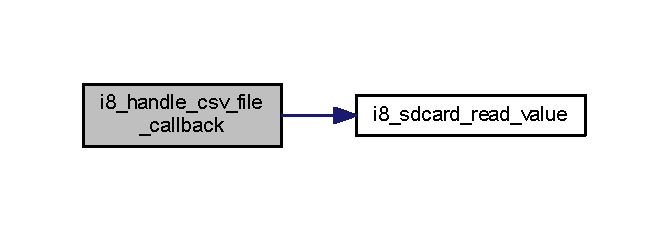
\includegraphics[width=321pt]{sd__app_8h_a5a7701bf6eb70c9a1ff531d3a7f687ab_cgraph}
\end{center}
\end{figure}
\mbox{\Hypertarget{sd__app_8h_ac64497358537694b4dd27b4cf9454015}\label{sd__app_8h_ac64497358537694b4dd27b4cf9454015}} 
\index{sd\+\_\+app.\+h@{sd\+\_\+app.\+h}!i8\+\_\+sdcard\+\_\+get\+\_\+channels\+\_\+flow@{i8\+\_\+sdcard\+\_\+get\+\_\+channels\+\_\+flow}}
\index{i8\+\_\+sdcard\+\_\+get\+\_\+channels\+\_\+flow@{i8\+\_\+sdcard\+\_\+get\+\_\+channels\+\_\+flow}!sd\+\_\+app.\+h@{sd\+\_\+app.\+h}}
\subsubsection{\texorpdfstring{i8\+\_\+sdcard\+\_\+get\+\_\+channels\+\_\+flow()}{i8\_sdcard\_get\_channels\_flow()}}
{\footnotesize\ttfamily int8\+\_\+t i8\+\_\+sdcard\+\_\+get\+\_\+channels\+\_\+flow (\begin{DoxyParamCaption}\item[{uint8\+\_\+t}]{u8\+\_\+location\+\_\+id,  }\item[{uint16\+\_\+t $\ast$}]{pu16\+\_\+channels\+\_\+flow }\end{DoxyParamCaption})}



get flow rate of 5 fertilizer channels flow meter for a given location 


\begin{DoxyParams}[1]{Parameters}
\mbox{\tt in}  & {\em u8\+\_\+location\+\_\+id} & Id of given location \\
\hline
\mbox{\tt out}  & {\em pu16\+\_\+channels\+\_\+flow} & flow rate \\
\hline
\end{DoxyParams}
\begin{DoxyReturn}{Returns}
0\+: read success -\/1\+: file is not exist -\/2\+: can not read 
\end{DoxyReturn}
Here is the call graph for this function\+:
\nopagebreak
\begin{figure}[H]
\begin{center}
\leavevmode
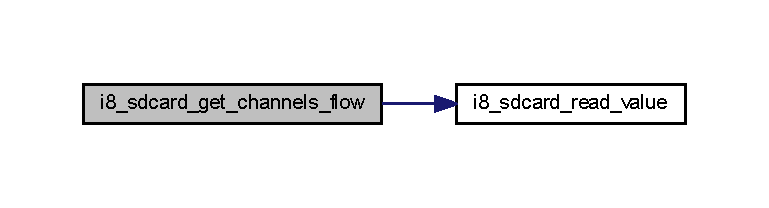
\includegraphics[width=350pt]{sd__app_8h_ac64497358537694b4dd27b4cf9454015_cgraph}
\end{center}
\end{figure}
\mbox{\Hypertarget{sd__app_8h_a4c963fbbe651d03d8982e219c4166e35}\label{sd__app_8h_a4c963fbbe651d03d8982e219c4166e35}} 
\index{sd\+\_\+app.\+h@{sd\+\_\+app.\+h}!i8\+\_\+sdcard\+\_\+get\+\_\+mainflow@{i8\+\_\+sdcard\+\_\+get\+\_\+mainflow}}
\index{i8\+\_\+sdcard\+\_\+get\+\_\+mainflow@{i8\+\_\+sdcard\+\_\+get\+\_\+mainflow}!sd\+\_\+app.\+h@{sd\+\_\+app.\+h}}
\subsubsection{\texorpdfstring{i8\+\_\+sdcard\+\_\+get\+\_\+mainflow()}{i8\_sdcard\_get\_mainflow()}}
{\footnotesize\ttfamily int8\+\_\+t i8\+\_\+sdcard\+\_\+get\+\_\+mainflow (\begin{DoxyParamCaption}\item[{uint8\+\_\+t}]{u8\+\_\+location\+\_\+id,  }\item[{uint32\+\_\+t $\ast$}]{pu32\+\_\+main\+\_\+flow }\end{DoxyParamCaption})}



get flow rate of main flow meter for a given location 


\begin{DoxyParams}[1]{Parameters}
\mbox{\tt in}  & {\em u8\+\_\+location\+\_\+id} & Id of given location \\
\hline
\mbox{\tt out}  & {\em pu32\+\_\+main\+\_\+flow} & flow rate (real value $\ast$ 10) Ex\+: the real value is 10.\+5m3/h =$>$ save value\+: 105 \\
\hline
\end{DoxyParams}
\begin{DoxyReturn}{Returns}
0\+: read success -\/1\+: file is not exist -\/2\+: can not read 
\end{DoxyReturn}
Here is the call graph for this function\+:
\nopagebreak
\begin{figure}[H]
\begin{center}
\leavevmode
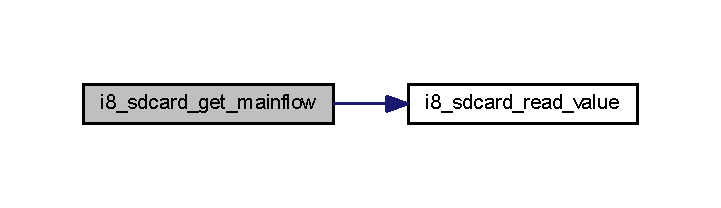
\includegraphics[width=346pt]{sd__app_8h_a4c963fbbe651d03d8982e219c4166e35_cgraph}
\end{center}
\end{figure}
\mbox{\Hypertarget{sd__app_8h_a33496be7efcfdf272994b216b05eb1f8}\label{sd__app_8h_a33496be7efcfdf272994b216b05eb1f8}} 
\index{sd\+\_\+app.\+h@{sd\+\_\+app.\+h}!i8\+\_\+sdcard\+\_\+get\+\_\+schedule\+\_\+version@{i8\+\_\+sdcard\+\_\+get\+\_\+schedule\+\_\+version}}
\index{i8\+\_\+sdcard\+\_\+get\+\_\+schedule\+\_\+version@{i8\+\_\+sdcard\+\_\+get\+\_\+schedule\+\_\+version}!sd\+\_\+app.\+h@{sd\+\_\+app.\+h}}
\subsubsection{\texorpdfstring{i8\+\_\+sdcard\+\_\+get\+\_\+schedule\+\_\+version()}{i8\_sdcard\_get\_schedule\_version()}}
{\footnotesize\ttfamily int8\+\_\+t i8\+\_\+sdcard\+\_\+get\+\_\+schedule\+\_\+version (\begin{DoxyParamCaption}\item[{char $\ast$}]{version }\end{DoxyParamCaption})}



get version of schedule file 


\begin{DoxyParams}[1]{Parameters}
\mbox{\tt out}  & {\em version} & version of schedule file \\
\hline
\end{DoxyParams}
\begin{DoxyReturn}{Returns}
0\+: read success -\/1\+: file is not exist -\/2\+: can not write 
\end{DoxyReturn}
Here is the call graph for this function\+:
\nopagebreak
\begin{figure}[H]
\begin{center}
\leavevmode
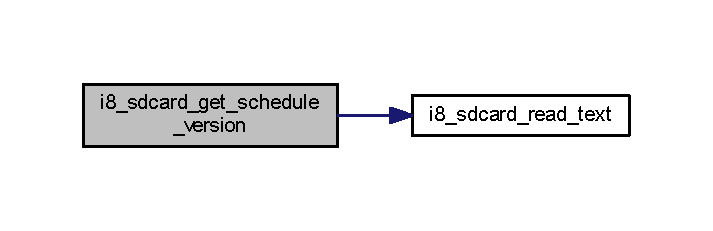
\includegraphics[width=342pt]{sd__app_8h_a33496be7efcfdf272994b216b05eb1f8_cgraph}
\end{center}
\end{figure}
\mbox{\Hypertarget{sd__app_8h_a2d21479adf7864569b3427aadc083579}\label{sd__app_8h_a2d21479adf7864569b3427aadc083579}} 
\index{sd\+\_\+app.\+h@{sd\+\_\+app.\+h}!i8\+\_\+sdcard\+\_\+save\+\_\+channels\+\_\+flow@{i8\+\_\+sdcard\+\_\+save\+\_\+channels\+\_\+flow}}
\index{i8\+\_\+sdcard\+\_\+save\+\_\+channels\+\_\+flow@{i8\+\_\+sdcard\+\_\+save\+\_\+channels\+\_\+flow}!sd\+\_\+app.\+h@{sd\+\_\+app.\+h}}
\subsubsection{\texorpdfstring{i8\+\_\+sdcard\+\_\+save\+\_\+channels\+\_\+flow()}{i8\_sdcard\_save\_channels\_flow()}}
{\footnotesize\ttfamily int8\+\_\+t i8\+\_\+sdcard\+\_\+save\+\_\+channels\+\_\+flow (\begin{DoxyParamCaption}\item[{uint8\+\_\+t}]{u8\+\_\+location\+\_\+id,  }\item[{uint16\+\_\+t $\ast$}]{pu16\+\_\+channels\+\_\+flow }\end{DoxyParamCaption})}



save flow rate of 5 fertilizer channels for a given location 


\begin{DoxyParams}[1]{Parameters}
\mbox{\tt in}  & {\em Id} & of given location \\
\hline
\mbox{\tt in}  & {\em pu16\+\_\+channels\+\_\+flow} & flow rate \\
\hline
\end{DoxyParams}
\begin{DoxyReturn}{Returns}
0\+: read success -\/1\+: file is not exist -\/2\+: can not write 
\end{DoxyReturn}
Here is the call graph for this function\+:
\nopagebreak
\begin{figure}[H]
\begin{center}
\leavevmode
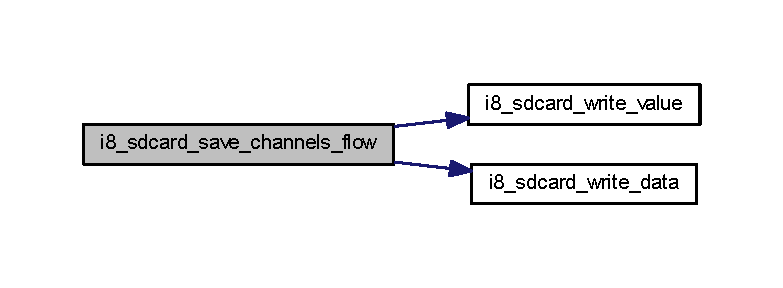
\includegraphics[width=350pt]{sd__app_8h_a2d21479adf7864569b3427aadc083579_cgraph}
\end{center}
\end{figure}
\mbox{\Hypertarget{sd__app_8h_a046dccab0a39863b7943a5e4aaf26298}\label{sd__app_8h_a046dccab0a39863b7943a5e4aaf26298}} 
\index{sd\+\_\+app.\+h@{sd\+\_\+app.\+h}!i8\+\_\+sdcard\+\_\+save\+\_\+mainflow@{i8\+\_\+sdcard\+\_\+save\+\_\+mainflow}}
\index{i8\+\_\+sdcard\+\_\+save\+\_\+mainflow@{i8\+\_\+sdcard\+\_\+save\+\_\+mainflow}!sd\+\_\+app.\+h@{sd\+\_\+app.\+h}}
\subsubsection{\texorpdfstring{i8\+\_\+sdcard\+\_\+save\+\_\+mainflow()}{i8\_sdcard\_save\_mainflow()}}
{\footnotesize\ttfamily int8\+\_\+t i8\+\_\+sdcard\+\_\+save\+\_\+mainflow (\begin{DoxyParamCaption}\item[{uint8\+\_\+t}]{u8\+\_\+location\+\_\+id,  }\item[{uint32\+\_\+t}]{u32\+\_\+main\+\_\+flow }\end{DoxyParamCaption})}



save flow rate of main flow meter for a given location 


\begin{DoxyParams}[1]{Parameters}
\mbox{\tt in}  & {\em u8\+\_\+location\+\_\+id} & Id of given location \\
\hline
\mbox{\tt in}  & {\em u32\+\_\+main\+\_\+flow} & flow rate (real value $\ast$ 10) Ex\+: the real value is 10.\+5m3/h =$>$ save value\+: 105 \\
\hline
\end{DoxyParams}
\begin{DoxyReturn}{Returns}
0\+: read success -\/1\+: file is not exist -\/2\+: can not write 
\end{DoxyReturn}
Here is the call graph for this function\+:
\nopagebreak
\begin{figure}[H]
\begin{center}
\leavevmode
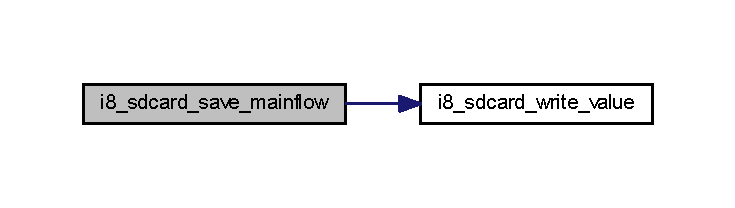
\includegraphics[width=350pt]{sd__app_8h_a046dccab0a39863b7943a5e4aaf26298_cgraph}
\end{center}
\end{figure}
\mbox{\Hypertarget{sd__app_8h_a47950b3f5c7eb8ba9316f92109afc47d}\label{sd__app_8h_a47950b3f5c7eb8ba9316f92109afc47d}} 
\index{sd\+\_\+app.\+h@{sd\+\_\+app.\+h}!i8\+\_\+sdcard\+\_\+save\+\_\+schedule\+\_\+version@{i8\+\_\+sdcard\+\_\+save\+\_\+schedule\+\_\+version}}
\index{i8\+\_\+sdcard\+\_\+save\+\_\+schedule\+\_\+version@{i8\+\_\+sdcard\+\_\+save\+\_\+schedule\+\_\+version}!sd\+\_\+app.\+h@{sd\+\_\+app.\+h}}
\subsubsection{\texorpdfstring{i8\+\_\+sdcard\+\_\+save\+\_\+schedule\+\_\+version()}{i8\_sdcard\_save\_schedule\_version()}}
{\footnotesize\ttfamily int8\+\_\+t i8\+\_\+sdcard\+\_\+save\+\_\+schedule\+\_\+version (\begin{DoxyParamCaption}\item[{char $\ast$}]{version }\end{DoxyParamCaption})}



save version of schedule file 


\begin{DoxyParams}[1]{Parameters}
\mbox{\tt in}  & {\em version} & version of schedule file \\
\hline
\end{DoxyParams}
\begin{DoxyReturn}{Returns}
0\+: read success -\/2\+: can not write 
\end{DoxyReturn}
Here is the call graph for this function\+:
\nopagebreak
\begin{figure}[H]
\begin{center}
\leavevmode
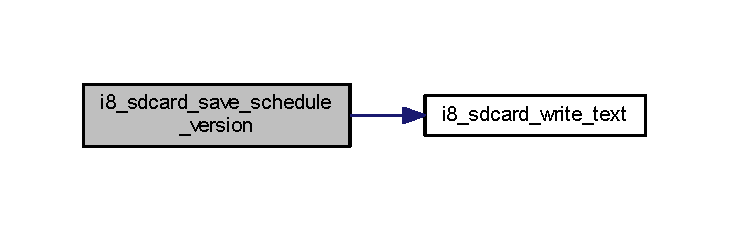
\includegraphics[width=350pt]{sd__app_8h_a47950b3f5c7eb8ba9316f92109afc47d_cgraph}
\end{center}
\end{figure}

\hypertarget{sd__manage__lib_8c}{}\section{sd\+\_\+manage\+\_\+lib.\+c File Reference}
\label{sd__manage__lib_8c}\index{sd\+\_\+manage\+\_\+lib.\+c@{sd\+\_\+manage\+\_\+lib.\+c}}


Contain functions to manage read and write sd card action.  


{\ttfamily \#include $<$stdint.\+h$>$}\newline
{\ttfamily \#include \char`\"{}sd\+\_\+manage\+\_\+lib.\+h\char`\"{}}\newline
{\ttfamily \#include \char`\"{}ff.\+h\char`\"{}}\newline
{\ttfamily \#include \char`\"{}H\+A\+L\+\_\+\+B\+S\+P.\+h\char`\"{}}\newline
{\ttfamily \#include \char`\"{}Free\+R\+T\+O\+S.\+h\char`\"{}}\newline
{\ttfamily \#include \char`\"{}task.\+h\char`\"{}}\newline
Include dependency graph for sd\+\_\+manage\+\_\+lib.\+c\+:
\nopagebreak
\begin{figure}[H]
\begin{center}
\leavevmode
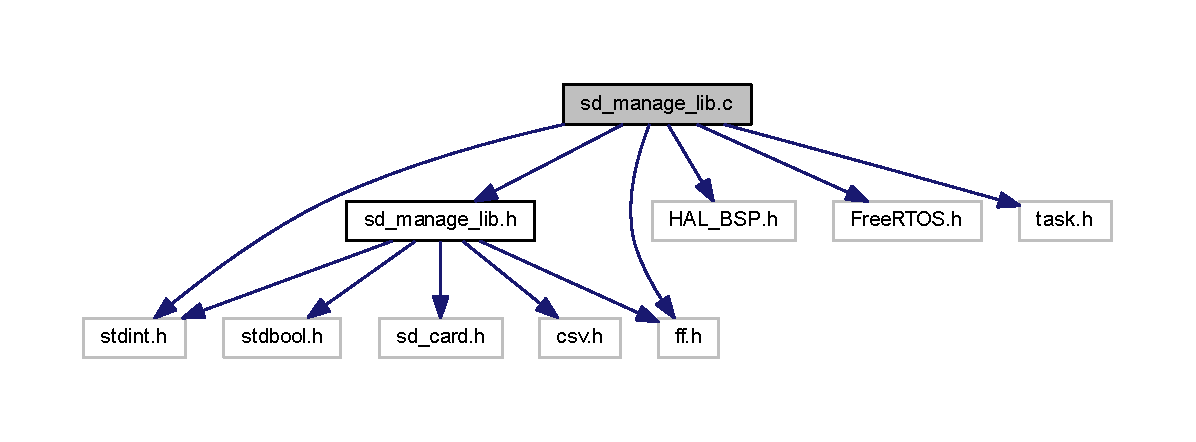
\includegraphics[width=350pt]{sd__manage__lib_8c__incl}
\end{center}
\end{figure}
\subsection*{Functions}
\begin{DoxyCompactItemize}
\item 
int8\+\_\+t \hyperlink{sd__manage__lib_8c_a37d4403b945bd02b8e8b17d5442f6166}{i8\+\_\+sdcard\+\_\+check\+\_\+exist\+\_\+file} (char $\ast$filename)
\begin{DoxyCompactList}\small\item\em Check a file is exist or not. \end{DoxyCompactList}\item 
int8\+\_\+t \hyperlink{sd__manage__lib_8c_a77f3c2ec2a0d177bb7954f338b8a1a9e}{i8\+\_\+sdcard\+\_\+delete\+\_\+file} (char $\ast$filename)
\begin{DoxyCompactList}\small\item\em Delete a file. \end{DoxyCompactList}\item 
int8\+\_\+t \hyperlink{sd__manage__lib_8c_a1a36bbc2e04b30e8b970a01d5bb5b6d8}{i8\+\_\+sdcard\+\_\+write\+\_\+value} (char $\ast$filename, uint32\+\_\+t u32\+\_\+addr, int32\+\_\+t i32\+\_\+value)
\begin{DoxyCompactList}\small\item\em Write a value to the given address in file. \end{DoxyCompactList}\item 
int8\+\_\+t \hyperlink{sd__manage__lib_8c_aa10f53e394fef9b6912012e17d93447c}{i8\+\_\+sdcard\+\_\+write\+\_\+data} (char $\ast$filename, uint32\+\_\+t u32\+\_\+addr, uint32\+\_\+t $\ast$u32\+\_\+data, uint32\+\_\+t u32\+\_\+len)
\begin{DoxyCompactList}\small\item\em Write a array of data to the given address in file. \end{DoxyCompactList}\item 
int8\+\_\+t \hyperlink{sd__manage__lib_8c_a81f7e2427d424cc9759559ba38f5b5e8}{i8\+\_\+sdcard\+\_\+write\+\_\+text} (char $\ast$filename, uint32\+\_\+t u32\+\_\+addr, char $\ast$c\+\_\+text)
\begin{DoxyCompactList}\small\item\em Write a string data the given address in file. \end{DoxyCompactList}\item 
int8\+\_\+t \hyperlink{sd__manage__lib_8c_a0567a8a5024b2dc8edddbee03677907e}{i8\+\_\+sdcard\+\_\+read\+\_\+value} (char $\ast$filename, uint32\+\_\+t u32\+\_\+addr, uint32\+\_\+t $\ast$pu32\+\_\+value)
\begin{DoxyCompactList}\small\item\em read a value from sd card \end{DoxyCompactList}\item 
int8\+\_\+t \hyperlink{sd__manage__lib_8c_af7ae9895e0278903d1bbd427b0d0f7d7}{i8\+\_\+sdcard\+\_\+read\+\_\+data} (char $\ast$filename, uint32\+\_\+t u32\+\_\+addr, uint32\+\_\+t $\ast$pu32\+\_\+data, uint32\+\_\+t u32\+\_\+len)
\begin{DoxyCompactList}\small\item\em read an array of data from sd card \end{DoxyCompactList}\item 
int8\+\_\+t \hyperlink{sd__manage__lib_8c_a6ca6542895c8b3d6a92f976b9343990d}{i8\+\_\+sdcard\+\_\+read\+\_\+text} (char $\ast$filename, uint32\+\_\+t u32\+\_\+addr, char $\ast$c\+\_\+text)
\begin{DoxyCompactList}\small\item\em read an array of data from sd card \end{DoxyCompactList}\item 
int8\+\_\+t \hyperlink{sd__manage__lib_8c_a681d1ddec3bf0fb2d85ca694c0017a87}{i8\+\_\+sdcard\+\_\+save\+\_\+file} (char $\ast$filename, const uint8\+\_\+t $\ast$pu8\+\_\+data, uint32\+\_\+t u32\+\_\+len)
\end{DoxyCompactItemize}


\subsection{Detailed Description}
Contain functions to manage read and write sd card action. 

\begin{DoxyAuthor}{Author}
Danh Pham 
\end{DoxyAuthor}
\begin{DoxyDate}{Date}
11 Nov 2020 
\end{DoxyDate}
\begin{DoxyVersion}{Version}
\+: 2.\+0.\+0 
\end{DoxyVersion}


\subsection{Function Documentation}
\mbox{\Hypertarget{sd__manage__lib_8c_a37d4403b945bd02b8e8b17d5442f6166}\label{sd__manage__lib_8c_a37d4403b945bd02b8e8b17d5442f6166}} 
\index{sd\+\_\+manage\+\_\+lib.\+c@{sd\+\_\+manage\+\_\+lib.\+c}!i8\+\_\+sdcard\+\_\+check\+\_\+exist\+\_\+file@{i8\+\_\+sdcard\+\_\+check\+\_\+exist\+\_\+file}}
\index{i8\+\_\+sdcard\+\_\+check\+\_\+exist\+\_\+file@{i8\+\_\+sdcard\+\_\+check\+\_\+exist\+\_\+file}!sd\+\_\+manage\+\_\+lib.\+c@{sd\+\_\+manage\+\_\+lib.\+c}}
\subsubsection{\texorpdfstring{i8\+\_\+sdcard\+\_\+check\+\_\+exist\+\_\+file()}{i8\_sdcard\_check\_exist\_file()}}
{\footnotesize\ttfamily int8\+\_\+t i8\+\_\+sdcard\+\_\+check\+\_\+exist\+\_\+file (\begin{DoxyParamCaption}\item[{char $\ast$}]{filename }\end{DoxyParamCaption})}



Check a file is exist or not. 

Add more include here

Variables declare

Private functions prototype

Public functions


\begin{DoxyParams}[1]{Parameters}
\mbox{\tt in}  & {\em filename} & name of file \\
\hline
\end{DoxyParams}
\begin{DoxyReturn}{Returns}
0\+: file is exist -\/1\+: file is not exist 
\end{DoxyReturn}
$<$file is not exist \mbox{\Hypertarget{sd__manage__lib_8c_a77f3c2ec2a0d177bb7954f338b8a1a9e}\label{sd__manage__lib_8c_a77f3c2ec2a0d177bb7954f338b8a1a9e}} 
\index{sd\+\_\+manage\+\_\+lib.\+c@{sd\+\_\+manage\+\_\+lib.\+c}!i8\+\_\+sdcard\+\_\+delete\+\_\+file@{i8\+\_\+sdcard\+\_\+delete\+\_\+file}}
\index{i8\+\_\+sdcard\+\_\+delete\+\_\+file@{i8\+\_\+sdcard\+\_\+delete\+\_\+file}!sd\+\_\+manage\+\_\+lib.\+c@{sd\+\_\+manage\+\_\+lib.\+c}}
\subsubsection{\texorpdfstring{i8\+\_\+sdcard\+\_\+delete\+\_\+file()}{i8\_sdcard\_delete\_file()}}
{\footnotesize\ttfamily int8\+\_\+t i8\+\_\+sdcard\+\_\+delete\+\_\+file (\begin{DoxyParamCaption}\item[{char $\ast$}]{filename }\end{DoxyParamCaption})}



Delete a file. 


\begin{DoxyParams}[1]{Parameters}
\mbox{\tt in}  & {\em filename} & name of file \\
\hline
\end{DoxyParams}
\begin{DoxyReturn}{Returns}
0\+: delete success or file is not exist -\/2\+: can not delete 
\end{DoxyReturn}
$<$file is not exist \mbox{\Hypertarget{sd__manage__lib_8c_af7ae9895e0278903d1bbd427b0d0f7d7}\label{sd__manage__lib_8c_af7ae9895e0278903d1bbd427b0d0f7d7}} 
\index{sd\+\_\+manage\+\_\+lib.\+c@{sd\+\_\+manage\+\_\+lib.\+c}!i8\+\_\+sdcard\+\_\+read\+\_\+data@{i8\+\_\+sdcard\+\_\+read\+\_\+data}}
\index{i8\+\_\+sdcard\+\_\+read\+\_\+data@{i8\+\_\+sdcard\+\_\+read\+\_\+data}!sd\+\_\+manage\+\_\+lib.\+c@{sd\+\_\+manage\+\_\+lib.\+c}}
\subsubsection{\texorpdfstring{i8\+\_\+sdcard\+\_\+read\+\_\+data()}{i8\_sdcard\_read\_data()}}
{\footnotesize\ttfamily i8\+\_\+sdcard\+\_\+read\+\_\+data (\begin{DoxyParamCaption}\item[{char $\ast$}]{filename,  }\item[{uint32\+\_\+t}]{u32\+\_\+addr,  }\item[{uint32\+\_\+t $\ast$}]{pu32\+\_\+data,  }\item[{uint32\+\_\+t}]{u32\+\_\+len }\end{DoxyParamCaption})}



read an array of data from sd card 


\begin{DoxyParams}[1]{Parameters}
\mbox{\tt in}  & {\em filename} & name of file \\
\hline
\mbox{\tt in}  & {\em u32\+\_\+addr} & address to read \\
\hline
\mbox{\tt out}  & {\em pu32\+\_\+data} & buffer of data \\
\hline
\mbox{\tt in}  & {\em u32\+\_\+len} & length of data \\
\hline
\end{DoxyParams}
\begin{DoxyReturn}{Returns}
0\+: read success -\/1\+: file is not exist -\/2\+: can not read 
\end{DoxyReturn}
\mbox{\Hypertarget{sd__manage__lib_8c_a6ca6542895c8b3d6a92f976b9343990d}\label{sd__manage__lib_8c_a6ca6542895c8b3d6a92f976b9343990d}} 
\index{sd\+\_\+manage\+\_\+lib.\+c@{sd\+\_\+manage\+\_\+lib.\+c}!i8\+\_\+sdcard\+\_\+read\+\_\+text@{i8\+\_\+sdcard\+\_\+read\+\_\+text}}
\index{i8\+\_\+sdcard\+\_\+read\+\_\+text@{i8\+\_\+sdcard\+\_\+read\+\_\+text}!sd\+\_\+manage\+\_\+lib.\+c@{sd\+\_\+manage\+\_\+lib.\+c}}
\subsubsection{\texorpdfstring{i8\+\_\+sdcard\+\_\+read\+\_\+text()}{i8\_sdcard\_read\_text()}}
{\footnotesize\ttfamily i8\+\_\+sdcard\+\_\+read\+\_\+text (\begin{DoxyParamCaption}\item[{char $\ast$}]{filename,  }\item[{uint32\+\_\+t}]{u32\+\_\+addr,  }\item[{char $\ast$}]{c\+\_\+text }\end{DoxyParamCaption})}



read an array of data from sd card 


\begin{DoxyParams}[1]{Parameters}
\mbox{\tt in}  & {\em filename} & name of file \\
\hline
\mbox{\tt in}  & {\em u32\+\_\+addr} & address to read \\
\hline
\mbox{\tt out}  & {\em c\+\_\+text} & buffer of text string \\
\hline
\end{DoxyParams}
\begin{DoxyReturn}{Returns}
0\+: read success -\/1\+: file is not exist -\/2\+: can not read 
\end{DoxyReturn}
Here is the caller graph for this function\+:
\nopagebreak
\begin{figure}[H]
\begin{center}
\leavevmode
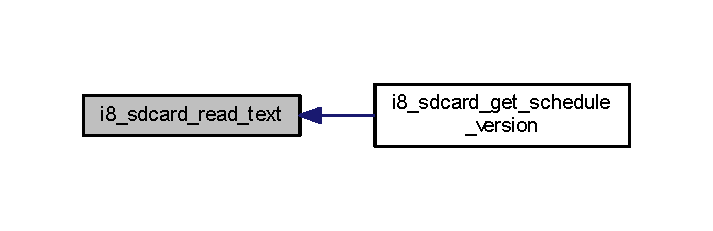
\includegraphics[width=342pt]{sd__manage__lib_8c_a6ca6542895c8b3d6a92f976b9343990d_icgraph}
\end{center}
\end{figure}
\mbox{\Hypertarget{sd__manage__lib_8c_a0567a8a5024b2dc8edddbee03677907e}\label{sd__manage__lib_8c_a0567a8a5024b2dc8edddbee03677907e}} 
\index{sd\+\_\+manage\+\_\+lib.\+c@{sd\+\_\+manage\+\_\+lib.\+c}!i8\+\_\+sdcard\+\_\+read\+\_\+value@{i8\+\_\+sdcard\+\_\+read\+\_\+value}}
\index{i8\+\_\+sdcard\+\_\+read\+\_\+value@{i8\+\_\+sdcard\+\_\+read\+\_\+value}!sd\+\_\+manage\+\_\+lib.\+c@{sd\+\_\+manage\+\_\+lib.\+c}}
\subsubsection{\texorpdfstring{i8\+\_\+sdcard\+\_\+read\+\_\+value()}{i8\_sdcard\_read\_value()}}
{\footnotesize\ttfamily i8\+\_\+sdcard\+\_\+read\+\_\+value (\begin{DoxyParamCaption}\item[{char $\ast$}]{filename,  }\item[{uint32\+\_\+t}]{u32\+\_\+addr,  }\item[{uint32\+\_\+t $\ast$}]{pu32\+\_\+value }\end{DoxyParamCaption})}



read a value from sd card 


\begin{DoxyParams}[1]{Parameters}
\mbox{\tt in}  & {\em filename} & name of file \\
\hline
\mbox{\tt in}  & {\em u32\+\_\+addr} & address to read \\
\hline
\mbox{\tt out}  & {\em pu32\+\_\+value} & buffer of value \\
\hline
\end{DoxyParams}
\begin{DoxyReturn}{Returns}
0\+: read success -\/1\+: file is not exist -\/2\+: can not read 
\end{DoxyReturn}
Here is the caller graph for this function\+:
\nopagebreak
\begin{figure}[H]
\begin{center}
\leavevmode
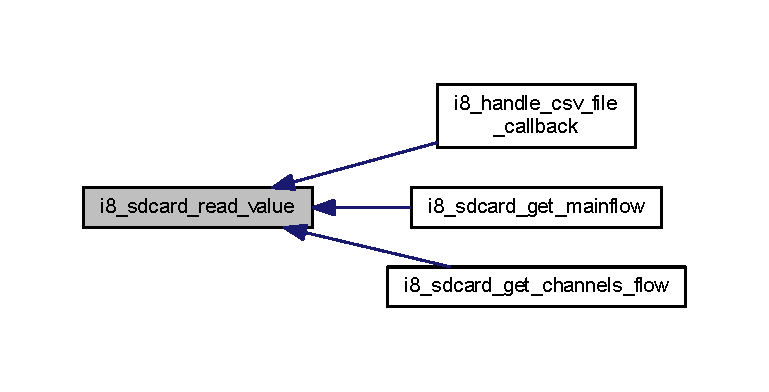
\includegraphics[width=350pt]{sd__manage__lib_8c_a0567a8a5024b2dc8edddbee03677907e_icgraph}
\end{center}
\end{figure}
\mbox{\Hypertarget{sd__manage__lib_8c_a681d1ddec3bf0fb2d85ca694c0017a87}\label{sd__manage__lib_8c_a681d1ddec3bf0fb2d85ca694c0017a87}} 
\index{sd\+\_\+manage\+\_\+lib.\+c@{sd\+\_\+manage\+\_\+lib.\+c}!i8\+\_\+sdcard\+\_\+save\+\_\+file@{i8\+\_\+sdcard\+\_\+save\+\_\+file}}
\index{i8\+\_\+sdcard\+\_\+save\+\_\+file@{i8\+\_\+sdcard\+\_\+save\+\_\+file}!sd\+\_\+manage\+\_\+lib.\+c@{sd\+\_\+manage\+\_\+lib.\+c}}
\subsubsection{\texorpdfstring{i8\+\_\+sdcard\+\_\+save\+\_\+file()}{i8\_sdcard\_save\_file()}}
{\footnotesize\ttfamily int8\+\_\+t i8\+\_\+sdcard\+\_\+save\+\_\+file (\begin{DoxyParamCaption}\item[{char $\ast$}]{filename,  }\item[{const uint8\+\_\+t $\ast$}]{pu8\+\_\+data,  }\item[{uint32\+\_\+t}]{u32\+\_\+len }\end{DoxyParamCaption})}

\mbox{\Hypertarget{sd__manage__lib_8c_aa10f53e394fef9b6912012e17d93447c}\label{sd__manage__lib_8c_aa10f53e394fef9b6912012e17d93447c}} 
\index{sd\+\_\+manage\+\_\+lib.\+c@{sd\+\_\+manage\+\_\+lib.\+c}!i8\+\_\+sdcard\+\_\+write\+\_\+data@{i8\+\_\+sdcard\+\_\+write\+\_\+data}}
\index{i8\+\_\+sdcard\+\_\+write\+\_\+data@{i8\+\_\+sdcard\+\_\+write\+\_\+data}!sd\+\_\+manage\+\_\+lib.\+c@{sd\+\_\+manage\+\_\+lib.\+c}}
\subsubsection{\texorpdfstring{i8\+\_\+sdcard\+\_\+write\+\_\+data()}{i8\_sdcard\_write\_data()}}
{\footnotesize\ttfamily i8\+\_\+sdcard\+\_\+write\+\_\+data (\begin{DoxyParamCaption}\item[{char $\ast$}]{filename,  }\item[{uint32\+\_\+t}]{u32\+\_\+addr,  }\item[{uint32\+\_\+t $\ast$}]{u32\+\_\+data,  }\item[{uint32\+\_\+t}]{u32\+\_\+len }\end{DoxyParamCaption})}



Write a array of data to the given address in file. 


\begin{DoxyParams}[1]{Parameters}
\mbox{\tt in}  & {\em filename} & name of file \\
\hline
\mbox{\tt in}  & {\em u32\+\_\+addr} & address to write, the address must divisible by 4 \\
\hline
\mbox{\tt in}  & {\em u32\+\_\+data} & data array to write \\
\hline
\mbox{\tt in}  & {\em u32\+\_\+len} & lenght of array \\
\hline
\end{DoxyParams}
\begin{DoxyReturn}{Returns}
0\+: write success -\/1\+: file is not exist -\/2\+: can not write 
\end{DoxyReturn}
$<$file is not exist Here is the caller graph for this function\+:
\nopagebreak
\begin{figure}[H]
\begin{center}
\leavevmode
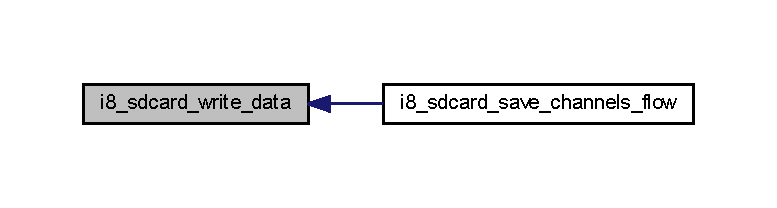
\includegraphics[width=350pt]{sd__manage__lib_8c_aa10f53e394fef9b6912012e17d93447c_icgraph}
\end{center}
\end{figure}
\mbox{\Hypertarget{sd__manage__lib_8c_a81f7e2427d424cc9759559ba38f5b5e8}\label{sd__manage__lib_8c_a81f7e2427d424cc9759559ba38f5b5e8}} 
\index{sd\+\_\+manage\+\_\+lib.\+c@{sd\+\_\+manage\+\_\+lib.\+c}!i8\+\_\+sdcard\+\_\+write\+\_\+text@{i8\+\_\+sdcard\+\_\+write\+\_\+text}}
\index{i8\+\_\+sdcard\+\_\+write\+\_\+text@{i8\+\_\+sdcard\+\_\+write\+\_\+text}!sd\+\_\+manage\+\_\+lib.\+c@{sd\+\_\+manage\+\_\+lib.\+c}}
\subsubsection{\texorpdfstring{i8\+\_\+sdcard\+\_\+write\+\_\+text()}{i8\_sdcard\_write\_text()}}
{\footnotesize\ttfamily int8\+\_\+t i8\+\_\+sdcard\+\_\+write\+\_\+text (\begin{DoxyParamCaption}\item[{char $\ast$}]{filename,  }\item[{uint32\+\_\+t}]{u32\+\_\+addr,  }\item[{char $\ast$}]{c\+\_\+text }\end{DoxyParamCaption})}



Write a string data the given address in file. 


\begin{DoxyParams}[1]{Parameters}
\mbox{\tt in}  & {\em filename} & name of file \\
\hline
\mbox{\tt in}  & {\em u32\+\_\+addr} & address to write \\
\hline
\mbox{\tt in}  & {\em c\+\_\+text} & string write \\
\hline
\end{DoxyParams}
\begin{DoxyReturn}{Returns}
0\+: write success -\/1\+: file is not exist -\/2\+: can not write 
\end{DoxyReturn}
Here is the caller graph for this function\+:
\nopagebreak
\begin{figure}[H]
\begin{center}
\leavevmode
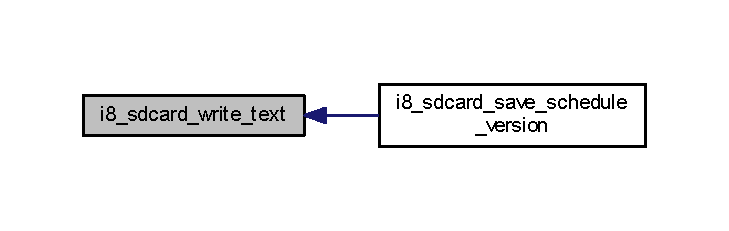
\includegraphics[width=350pt]{sd__manage__lib_8c_a81f7e2427d424cc9759559ba38f5b5e8_icgraph}
\end{center}
\end{figure}
\mbox{\Hypertarget{sd__manage__lib_8c_a1a36bbc2e04b30e8b970a01d5bb5b6d8}\label{sd__manage__lib_8c_a1a36bbc2e04b30e8b970a01d5bb5b6d8}} 
\index{sd\+\_\+manage\+\_\+lib.\+c@{sd\+\_\+manage\+\_\+lib.\+c}!i8\+\_\+sdcard\+\_\+write\+\_\+value@{i8\+\_\+sdcard\+\_\+write\+\_\+value}}
\index{i8\+\_\+sdcard\+\_\+write\+\_\+value@{i8\+\_\+sdcard\+\_\+write\+\_\+value}!sd\+\_\+manage\+\_\+lib.\+c@{sd\+\_\+manage\+\_\+lib.\+c}}
\subsubsection{\texorpdfstring{i8\+\_\+sdcard\+\_\+write\+\_\+value()}{i8\_sdcard\_write\_value()}}
{\footnotesize\ttfamily i8\+\_\+sdcard\+\_\+write\+\_\+value (\begin{DoxyParamCaption}\item[{char $\ast$}]{filename,  }\item[{uint32\+\_\+t}]{u32\+\_\+addr,  }\item[{int32\+\_\+t}]{i32\+\_\+value }\end{DoxyParamCaption})}



Write a value to the given address in file. 


\begin{DoxyParams}[1]{Parameters}
\mbox{\tt in}  & {\em filename} & name of file \\
\hline
\mbox{\tt in}  & {\em u32\+\_\+addr} & address to write, the address must divisible by 4 \\
\hline
\mbox{\tt in}  & {\em i32\+\_\+value} & value to write \\
\hline
\end{DoxyParams}
\begin{DoxyReturn}{Returns}
0\+: write success -\/1\+: file is not exist -\/2\+: can not write 
\end{DoxyReturn}
$<$file is not exist Here is the caller graph for this function\+:
\nopagebreak
\begin{figure}[H]
\begin{center}
\leavevmode
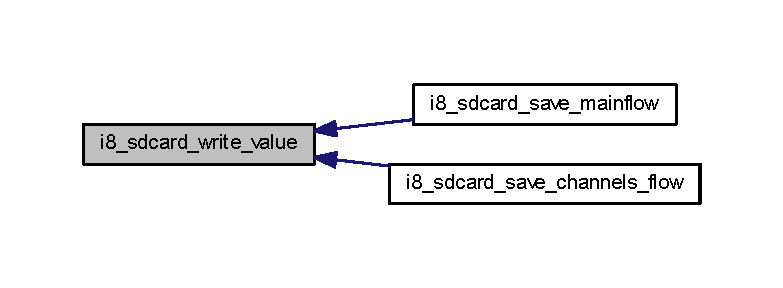
\includegraphics[width=350pt]{sd__manage__lib_8c_a1a36bbc2e04b30e8b970a01d5bb5b6d8_icgraph}
\end{center}
\end{figure}

\hypertarget{sd__manage__lib_8h}{}\section{sd\+\_\+manage\+\_\+lib.\+h File Reference}
\label{sd__manage__lib_8h}\index{sd\+\_\+manage\+\_\+lib.\+h@{sd\+\_\+manage\+\_\+lib.\+h}}
{\ttfamily \#include $<$stdint.\+h$>$}\newline
{\ttfamily \#include $<$stdbool.\+h$>$}\newline
{\ttfamily \#include \char`\"{}ff.\+h\char`\"{}}\newline
{\ttfamily \#include \char`\"{}sd\+\_\+card.\+h\char`\"{}}\newline
{\ttfamily \#include \char`\"{}csv.\+h\char`\"{}}\newline
Include dependency graph for sd\+\_\+manage\+\_\+lib.\+h\+:
\nopagebreak
\begin{figure}[H]
\begin{center}
\leavevmode
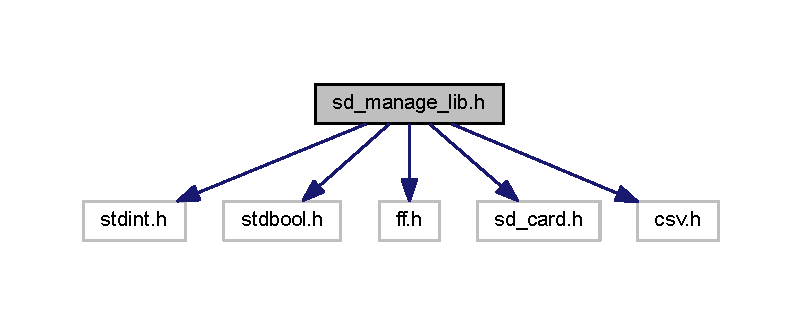
\includegraphics[width=350pt]{sd__manage__lib_8h__incl}
\end{center}
\end{figure}
This graph shows which files directly or indirectly include this file\+:
\nopagebreak
\begin{figure}[H]
\begin{center}
\leavevmode
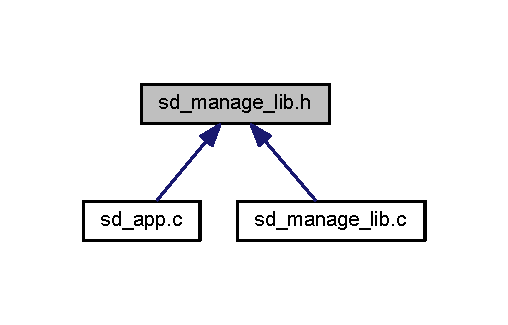
\includegraphics[width=244pt]{sd__manage__lib_8h__dep__incl}
\end{center}
\end{figure}
\subsection*{Classes}
\begin{DoxyCompactItemize}
\item 
struct \hyperlink{struct_s_t_r_u___c_s_v___c_o_u_n_t}{S\+T\+R\+U\+\_\+\+C\+S\+V\+\_\+\+C\+O\+U\+NT}
\end{DoxyCompactItemize}
\subsection*{Macros}
\begin{DoxyCompactItemize}
\item 
\#define \hyperlink{sd__manage__lib_8h_aee0f936ed68d37e2cf4b68650673a655}{S\+D\+\_\+\+T\+A\+K\+E\+\_\+\+S\+E\+M\+A\+P\+H\+O\+R\+E\+\_\+\+T\+I\+M\+E\+O\+UT}~(5)
\item 
\#define \hyperlink{sd__manage__lib_8h_a88494b7e34c7201cd4650e4c66fe357f}{W\+R\+I\+T\+E\+\_\+\+SD}~(0)
\item 
\#define \hyperlink{sd__manage__lib_8h_ab8498f40965c76452e3abd5c38bb3652}{R\+E\+A\+D\+\_\+\+SD}~(1)
\item 
\#define \hyperlink{sd__manage__lib_8h_a5bdc195dc5763a801ec3cd4bf8f448c9}{S\+D\+\_\+\+OK}~(0)
\item 
\#define \hyperlink{sd__manage__lib_8h_a67e0fc42bd2a57d3452e6a1315a618d7}{M\+A\+X\+\_\+\+S\+D\+\_\+\+T\+E\+X\+T\+\_\+\+L\+EN}~(30)
\end{DoxyCompactItemize}
\subsection*{Functions}
\begin{DoxyCompactItemize}
\item 
int8\+\_\+t \hyperlink{sd__manage__lib_8h_a37d4403b945bd02b8e8b17d5442f6166}{i8\+\_\+sdcard\+\_\+check\+\_\+exist\+\_\+file} (char $\ast$filename)
\begin{DoxyCompactList}\small\item\em Check a file is exist or not. \end{DoxyCompactList}\item 
int8\+\_\+t \hyperlink{sd__manage__lib_8h_a77f3c2ec2a0d177bb7954f338b8a1a9e}{i8\+\_\+sdcard\+\_\+delete\+\_\+file} (char $\ast$filename)
\begin{DoxyCompactList}\small\item\em Delete a file. \end{DoxyCompactList}\item 
int8\+\_\+t \hyperlink{sd__manage__lib_8h_a132824b2516bca9a4c4994c4ec17ad54}{i8\+\_\+sdcard\+\_\+write\+\_\+value} (char $\ast$filename, uint32\+\_\+t u32\+\_\+addr, int32\+\_\+t i32\+\_\+value)
\begin{DoxyCompactList}\small\item\em Write a value to the given address in file. \end{DoxyCompactList}\item 
int8\+\_\+t \hyperlink{sd__manage__lib_8h_a9a526861ab82b18d6e3f4d46aac1579e}{i8\+\_\+sdcard\+\_\+write\+\_\+data} (char $\ast$filename, uint32\+\_\+t u32\+\_\+addr, uint32\+\_\+t $\ast$u32\+\_\+data, uint32\+\_\+t u32\+\_\+len)
\begin{DoxyCompactList}\small\item\em Write a array of data to the given address in file. \end{DoxyCompactList}\item 
int8\+\_\+t \hyperlink{sd__manage__lib_8h_a81f7e2427d424cc9759559ba38f5b5e8}{i8\+\_\+sdcard\+\_\+write\+\_\+text} (char $\ast$filename, uint32\+\_\+t u32\+\_\+addr, char $\ast$c\+\_\+text)
\begin{DoxyCompactList}\small\item\em Write a string data the given address in file. \end{DoxyCompactList}\item 
int8\+\_\+t \hyperlink{sd__manage__lib_8h_a50052563122365fef8bf88a9292010f6}{i8\+\_\+sdcard\+\_\+read\+\_\+value} (char $\ast$filename, uint32\+\_\+t u32\+\_\+addr, uint32\+\_\+t $\ast$pu32\+\_\+value)
\begin{DoxyCompactList}\small\item\em read a value from sd card \end{DoxyCompactList}\item 
int8\+\_\+t \hyperlink{sd__manage__lib_8h_a4430e4d8b7bd7ab20a7a1a66a7f43fa4}{i8\+\_\+sdcard\+\_\+read\+\_\+data} (char $\ast$filename, uint32\+\_\+t u32\+\_\+addr, uint32\+\_\+t $\ast$pu32\+\_\+data, uint32\+\_\+t u32\+\_\+len)
\begin{DoxyCompactList}\small\item\em read an array of data from sd card \end{DoxyCompactList}\item 
int8\+\_\+t \hyperlink{sd__manage__lib_8h_aebb9cf3858c452a21d5b558670b3b1ca}{i8\+\_\+sdcard\+\_\+read\+\_\+text} (char $\ast$filename, uint32\+\_\+t u32\+\_\+addr, char $\ast$c\+\_\+text)
\begin{DoxyCompactList}\small\item\em read an array of data from sd card \end{DoxyCompactList}\item 
int8\+\_\+t \hyperlink{sd__manage__lib_8h_a681d1ddec3bf0fb2d85ca694c0017a87}{i8\+\_\+sdcard\+\_\+save\+\_\+file} (char $\ast$filename, const uint8\+\_\+t $\ast$pu8\+\_\+data, uint32\+\_\+t u32\+\_\+len)
\end{DoxyCompactItemize}


\subsection{Macro Definition Documentation}
\mbox{\Hypertarget{sd__manage__lib_8h_a67e0fc42bd2a57d3452e6a1315a618d7}\label{sd__manage__lib_8h_a67e0fc42bd2a57d3452e6a1315a618d7}} 
\index{sd\+\_\+manage\+\_\+lib.\+h@{sd\+\_\+manage\+\_\+lib.\+h}!M\+A\+X\+\_\+\+S\+D\+\_\+\+T\+E\+X\+T\+\_\+\+L\+EN@{M\+A\+X\+\_\+\+S\+D\+\_\+\+T\+E\+X\+T\+\_\+\+L\+EN}}
\index{M\+A\+X\+\_\+\+S\+D\+\_\+\+T\+E\+X\+T\+\_\+\+L\+EN@{M\+A\+X\+\_\+\+S\+D\+\_\+\+T\+E\+X\+T\+\_\+\+L\+EN}!sd\+\_\+manage\+\_\+lib.\+h@{sd\+\_\+manage\+\_\+lib.\+h}}
\subsubsection{\texorpdfstring{M\+A\+X\+\_\+\+S\+D\+\_\+\+T\+E\+X\+T\+\_\+\+L\+EN}{MAX\_SD\_TEXT\_LEN}}
{\footnotesize\ttfamily \#define M\+A\+X\+\_\+\+S\+D\+\_\+\+T\+E\+X\+T\+\_\+\+L\+EN~(30)}

Maximum length of text to save/load from sd card \mbox{\Hypertarget{sd__manage__lib_8h_ab8498f40965c76452e3abd5c38bb3652}\label{sd__manage__lib_8h_ab8498f40965c76452e3abd5c38bb3652}} 
\index{sd\+\_\+manage\+\_\+lib.\+h@{sd\+\_\+manage\+\_\+lib.\+h}!R\+E\+A\+D\+\_\+\+SD@{R\+E\+A\+D\+\_\+\+SD}}
\index{R\+E\+A\+D\+\_\+\+SD@{R\+E\+A\+D\+\_\+\+SD}!sd\+\_\+manage\+\_\+lib.\+h@{sd\+\_\+manage\+\_\+lib.\+h}}
\subsubsection{\texorpdfstring{R\+E\+A\+D\+\_\+\+SD}{READ\_SD}}
{\footnotesize\ttfamily \#define R\+E\+A\+D\+\_\+\+SD~(1)}

Macro to read SD card \mbox{\Hypertarget{sd__manage__lib_8h_a5bdc195dc5763a801ec3cd4bf8f448c9}\label{sd__manage__lib_8h_a5bdc195dc5763a801ec3cd4bf8f448c9}} 
\index{sd\+\_\+manage\+\_\+lib.\+h@{sd\+\_\+manage\+\_\+lib.\+h}!S\+D\+\_\+\+OK@{S\+D\+\_\+\+OK}}
\index{S\+D\+\_\+\+OK@{S\+D\+\_\+\+OK}!sd\+\_\+manage\+\_\+lib.\+h@{sd\+\_\+manage\+\_\+lib.\+h}}
\subsubsection{\texorpdfstring{S\+D\+\_\+\+OK}{SD\_OK}}
{\footnotesize\ttfamily \#define S\+D\+\_\+\+OK~(0)}

Result of read/write process \mbox{\Hypertarget{sd__manage__lib_8h_aee0f936ed68d37e2cf4b68650673a655}\label{sd__manage__lib_8h_aee0f936ed68d37e2cf4b68650673a655}} 
\index{sd\+\_\+manage\+\_\+lib.\+h@{sd\+\_\+manage\+\_\+lib.\+h}!S\+D\+\_\+\+T\+A\+K\+E\+\_\+\+S\+E\+M\+A\+P\+H\+O\+R\+E\+\_\+\+T\+I\+M\+E\+O\+UT@{S\+D\+\_\+\+T\+A\+K\+E\+\_\+\+S\+E\+M\+A\+P\+H\+O\+R\+E\+\_\+\+T\+I\+M\+E\+O\+UT}}
\index{S\+D\+\_\+\+T\+A\+K\+E\+\_\+\+S\+E\+M\+A\+P\+H\+O\+R\+E\+\_\+\+T\+I\+M\+E\+O\+UT@{S\+D\+\_\+\+T\+A\+K\+E\+\_\+\+S\+E\+M\+A\+P\+H\+O\+R\+E\+\_\+\+T\+I\+M\+E\+O\+UT}!sd\+\_\+manage\+\_\+lib.\+h@{sd\+\_\+manage\+\_\+lib.\+h}}
\subsubsection{\texorpdfstring{S\+D\+\_\+\+T\+A\+K\+E\+\_\+\+S\+E\+M\+A\+P\+H\+O\+R\+E\+\_\+\+T\+I\+M\+E\+O\+UT}{SD\_TAKE\_SEMAPHORE\_TIMEOUT}}
{\footnotesize\ttfamily \#define S\+D\+\_\+\+T\+A\+K\+E\+\_\+\+S\+E\+M\+A\+P\+H\+O\+R\+E\+\_\+\+T\+I\+M\+E\+O\+UT~(5)}

Time to wait semaphore \mbox{\Hypertarget{sd__manage__lib_8h_a88494b7e34c7201cd4650e4c66fe357f}\label{sd__manage__lib_8h_a88494b7e34c7201cd4650e4c66fe357f}} 
\index{sd\+\_\+manage\+\_\+lib.\+h@{sd\+\_\+manage\+\_\+lib.\+h}!W\+R\+I\+T\+E\+\_\+\+SD@{W\+R\+I\+T\+E\+\_\+\+SD}}
\index{W\+R\+I\+T\+E\+\_\+\+SD@{W\+R\+I\+T\+E\+\_\+\+SD}!sd\+\_\+manage\+\_\+lib.\+h@{sd\+\_\+manage\+\_\+lib.\+h}}
\subsubsection{\texorpdfstring{W\+R\+I\+T\+E\+\_\+\+SD}{WRITE\_SD}}
{\footnotesize\ttfamily \#define W\+R\+I\+T\+E\+\_\+\+SD~(0)}

Macro to write SD card 

\subsection{Function Documentation}
\mbox{\Hypertarget{sd__manage__lib_8h_a37d4403b945bd02b8e8b17d5442f6166}\label{sd__manage__lib_8h_a37d4403b945bd02b8e8b17d5442f6166}} 
\index{sd\+\_\+manage\+\_\+lib.\+h@{sd\+\_\+manage\+\_\+lib.\+h}!i8\+\_\+sdcard\+\_\+check\+\_\+exist\+\_\+file@{i8\+\_\+sdcard\+\_\+check\+\_\+exist\+\_\+file}}
\index{i8\+\_\+sdcard\+\_\+check\+\_\+exist\+\_\+file@{i8\+\_\+sdcard\+\_\+check\+\_\+exist\+\_\+file}!sd\+\_\+manage\+\_\+lib.\+h@{sd\+\_\+manage\+\_\+lib.\+h}}
\subsubsection{\texorpdfstring{i8\+\_\+sdcard\+\_\+check\+\_\+exist\+\_\+file()}{i8\_sdcard\_check\_exist\_file()}}
{\footnotesize\ttfamily int8\+\_\+t i8\+\_\+sdcard\+\_\+check\+\_\+exist\+\_\+file (\begin{DoxyParamCaption}\item[{char $\ast$}]{filename }\end{DoxyParamCaption})}



Check a file is exist or not. 

Extern functions

Add more include here

Variables declare

Private functions prototype

Public functions


\begin{DoxyParams}[1]{Parameters}
\mbox{\tt in}  & {\em filename} & name of file \\
\hline
\end{DoxyParams}
\begin{DoxyReturn}{Returns}
0\+: file is exist -\/1\+: file is not exist 
\end{DoxyReturn}
$<$file is not exist \mbox{\Hypertarget{sd__manage__lib_8h_a77f3c2ec2a0d177bb7954f338b8a1a9e}\label{sd__manage__lib_8h_a77f3c2ec2a0d177bb7954f338b8a1a9e}} 
\index{sd\+\_\+manage\+\_\+lib.\+h@{sd\+\_\+manage\+\_\+lib.\+h}!i8\+\_\+sdcard\+\_\+delete\+\_\+file@{i8\+\_\+sdcard\+\_\+delete\+\_\+file}}
\index{i8\+\_\+sdcard\+\_\+delete\+\_\+file@{i8\+\_\+sdcard\+\_\+delete\+\_\+file}!sd\+\_\+manage\+\_\+lib.\+h@{sd\+\_\+manage\+\_\+lib.\+h}}
\subsubsection{\texorpdfstring{i8\+\_\+sdcard\+\_\+delete\+\_\+file()}{i8\_sdcard\_delete\_file()}}
{\footnotesize\ttfamily int8\+\_\+t i8\+\_\+sdcard\+\_\+delete\+\_\+file (\begin{DoxyParamCaption}\item[{char $\ast$}]{filename }\end{DoxyParamCaption})}



Delete a file. 


\begin{DoxyParams}[1]{Parameters}
\mbox{\tt in}  & {\em filename} & name of file \\
\hline
\end{DoxyParams}
\begin{DoxyReturn}{Returns}
0\+: delete success or file is not exist -\/2\+: can not delete 
\end{DoxyReturn}
$<$file is not exist \mbox{\Hypertarget{sd__manage__lib_8h_a4430e4d8b7bd7ab20a7a1a66a7f43fa4}\label{sd__manage__lib_8h_a4430e4d8b7bd7ab20a7a1a66a7f43fa4}} 
\index{sd\+\_\+manage\+\_\+lib.\+h@{sd\+\_\+manage\+\_\+lib.\+h}!i8\+\_\+sdcard\+\_\+read\+\_\+data@{i8\+\_\+sdcard\+\_\+read\+\_\+data}}
\index{i8\+\_\+sdcard\+\_\+read\+\_\+data@{i8\+\_\+sdcard\+\_\+read\+\_\+data}!sd\+\_\+manage\+\_\+lib.\+h@{sd\+\_\+manage\+\_\+lib.\+h}}
\subsubsection{\texorpdfstring{i8\+\_\+sdcard\+\_\+read\+\_\+data()}{i8\_sdcard\_read\_data()}}
{\footnotesize\ttfamily int8\+\_\+t i8\+\_\+sdcard\+\_\+read\+\_\+data (\begin{DoxyParamCaption}\item[{char $\ast$}]{filename,  }\item[{uint32\+\_\+t}]{u32\+\_\+addr,  }\item[{uint32\+\_\+t $\ast$}]{pu32\+\_\+data,  }\item[{uint32\+\_\+t}]{u32\+\_\+len }\end{DoxyParamCaption})}



read an array of data from sd card 


\begin{DoxyParams}[1]{Parameters}
\mbox{\tt in}  & {\em filename} & name of file \\
\hline
\mbox{\tt in}  & {\em u32\+\_\+addr} & address to read \\
\hline
\mbox{\tt out}  & {\em pu32\+\_\+data} & buffer of data \\
\hline
\mbox{\tt in}  & {\em u32\+\_\+len} & length of data \\
\hline
\end{DoxyParams}
\begin{DoxyReturn}{Returns}
0\+: read success -\/1\+: file is not exist -\/2\+: can not read 
\end{DoxyReturn}
\mbox{\Hypertarget{sd__manage__lib_8h_aebb9cf3858c452a21d5b558670b3b1ca}\label{sd__manage__lib_8h_aebb9cf3858c452a21d5b558670b3b1ca}} 
\index{sd\+\_\+manage\+\_\+lib.\+h@{sd\+\_\+manage\+\_\+lib.\+h}!i8\+\_\+sdcard\+\_\+read\+\_\+text@{i8\+\_\+sdcard\+\_\+read\+\_\+text}}
\index{i8\+\_\+sdcard\+\_\+read\+\_\+text@{i8\+\_\+sdcard\+\_\+read\+\_\+text}!sd\+\_\+manage\+\_\+lib.\+h@{sd\+\_\+manage\+\_\+lib.\+h}}
\subsubsection{\texorpdfstring{i8\+\_\+sdcard\+\_\+read\+\_\+text()}{i8\_sdcard\_read\_text()}}
{\footnotesize\ttfamily int8\+\_\+t i8\+\_\+sdcard\+\_\+read\+\_\+text (\begin{DoxyParamCaption}\item[{char $\ast$}]{filename,  }\item[{uint32\+\_\+t}]{u32\+\_\+addr,  }\item[{char $\ast$}]{c\+\_\+text }\end{DoxyParamCaption})}



read an array of data from sd card 


\begin{DoxyParams}[1]{Parameters}
\mbox{\tt in}  & {\em filename} & name of file \\
\hline
\mbox{\tt in}  & {\em u32\+\_\+addr} & address to read \\
\hline
\mbox{\tt out}  & {\em c\+\_\+text} & buffer of text string \\
\hline
\end{DoxyParams}
\begin{DoxyReturn}{Returns}
0\+: read success -\/1\+: file is not exist -\/2\+: can not read 
\end{DoxyReturn}
Here is the caller graph for this function\+:
\nopagebreak
\begin{figure}[H]
\begin{center}
\leavevmode
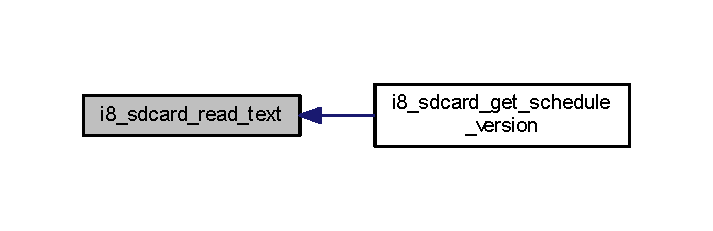
\includegraphics[width=342pt]{sd__manage__lib_8h_aebb9cf3858c452a21d5b558670b3b1ca_icgraph}
\end{center}
\end{figure}
\mbox{\Hypertarget{sd__manage__lib_8h_a50052563122365fef8bf88a9292010f6}\label{sd__manage__lib_8h_a50052563122365fef8bf88a9292010f6}} 
\index{sd\+\_\+manage\+\_\+lib.\+h@{sd\+\_\+manage\+\_\+lib.\+h}!i8\+\_\+sdcard\+\_\+read\+\_\+value@{i8\+\_\+sdcard\+\_\+read\+\_\+value}}
\index{i8\+\_\+sdcard\+\_\+read\+\_\+value@{i8\+\_\+sdcard\+\_\+read\+\_\+value}!sd\+\_\+manage\+\_\+lib.\+h@{sd\+\_\+manage\+\_\+lib.\+h}}
\subsubsection{\texorpdfstring{i8\+\_\+sdcard\+\_\+read\+\_\+value()}{i8\_sdcard\_read\_value()}}
{\footnotesize\ttfamily int8\+\_\+t i8\+\_\+sdcard\+\_\+read\+\_\+value (\begin{DoxyParamCaption}\item[{char $\ast$}]{filename,  }\item[{uint32\+\_\+t}]{u32\+\_\+addr,  }\item[{uint32\+\_\+t $\ast$}]{pu32\+\_\+value }\end{DoxyParamCaption})}



read a value from sd card 


\begin{DoxyParams}[1]{Parameters}
\mbox{\tt in}  & {\em filename} & name of file \\
\hline
\mbox{\tt in}  & {\em u32\+\_\+addr} & address to read \\
\hline
\mbox{\tt out}  & {\em pu32\+\_\+value} & buffer of value \\
\hline
\end{DoxyParams}
\begin{DoxyReturn}{Returns}
0\+: read success -\/1\+: file is not exist -\/2\+: can not read 
\end{DoxyReturn}
Here is the caller graph for this function\+:
\nopagebreak
\begin{figure}[H]
\begin{center}
\leavevmode
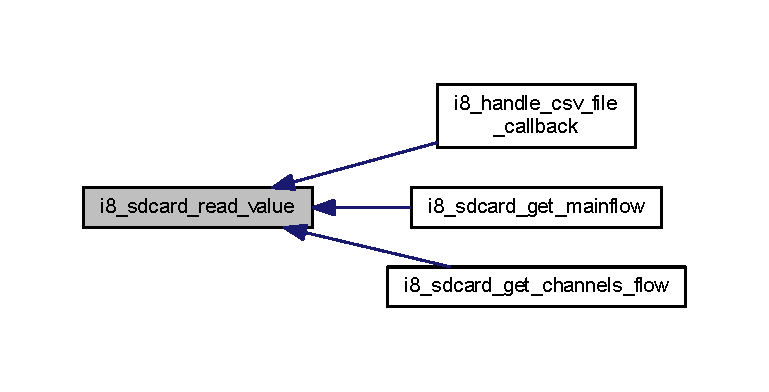
\includegraphics[width=350pt]{sd__manage__lib_8h_a50052563122365fef8bf88a9292010f6_icgraph}
\end{center}
\end{figure}
\mbox{\Hypertarget{sd__manage__lib_8h_a681d1ddec3bf0fb2d85ca694c0017a87}\label{sd__manage__lib_8h_a681d1ddec3bf0fb2d85ca694c0017a87}} 
\index{sd\+\_\+manage\+\_\+lib.\+h@{sd\+\_\+manage\+\_\+lib.\+h}!i8\+\_\+sdcard\+\_\+save\+\_\+file@{i8\+\_\+sdcard\+\_\+save\+\_\+file}}
\index{i8\+\_\+sdcard\+\_\+save\+\_\+file@{i8\+\_\+sdcard\+\_\+save\+\_\+file}!sd\+\_\+manage\+\_\+lib.\+h@{sd\+\_\+manage\+\_\+lib.\+h}}
\subsubsection{\texorpdfstring{i8\+\_\+sdcard\+\_\+save\+\_\+file()}{i8\_sdcard\_save\_file()}}
{\footnotesize\ttfamily int8\+\_\+t i8\+\_\+sdcard\+\_\+save\+\_\+file (\begin{DoxyParamCaption}\item[{char $\ast$}]{filename,  }\item[{const uint8\+\_\+t $\ast$}]{pu8\+\_\+data,  }\item[{uint32\+\_\+t}]{u32\+\_\+len }\end{DoxyParamCaption})}

\mbox{\Hypertarget{sd__manage__lib_8h_a9a526861ab82b18d6e3f4d46aac1579e}\label{sd__manage__lib_8h_a9a526861ab82b18d6e3f4d46aac1579e}} 
\index{sd\+\_\+manage\+\_\+lib.\+h@{sd\+\_\+manage\+\_\+lib.\+h}!i8\+\_\+sdcard\+\_\+write\+\_\+data@{i8\+\_\+sdcard\+\_\+write\+\_\+data}}
\index{i8\+\_\+sdcard\+\_\+write\+\_\+data@{i8\+\_\+sdcard\+\_\+write\+\_\+data}!sd\+\_\+manage\+\_\+lib.\+h@{sd\+\_\+manage\+\_\+lib.\+h}}
\subsubsection{\texorpdfstring{i8\+\_\+sdcard\+\_\+write\+\_\+data()}{i8\_sdcard\_write\_data()}}
{\footnotesize\ttfamily int8\+\_\+t i8\+\_\+sdcard\+\_\+write\+\_\+data (\begin{DoxyParamCaption}\item[{char $\ast$}]{filename,  }\item[{uint32\+\_\+t}]{u32\+\_\+addr,  }\item[{uint32\+\_\+t $\ast$}]{u32\+\_\+data,  }\item[{uint32\+\_\+t}]{u32\+\_\+len }\end{DoxyParamCaption})}



Write a array of data to the given address in file. 


\begin{DoxyParams}[1]{Parameters}
\mbox{\tt in}  & {\em filename} & name of file \\
\hline
\mbox{\tt in}  & {\em u32\+\_\+addr} & address to write, the address must divisible by 4 \\
\hline
\mbox{\tt in}  & {\em u32\+\_\+data} & data array to write \\
\hline
\mbox{\tt in}  & {\em u32\+\_\+len} & lenght of array \\
\hline
\end{DoxyParams}
\begin{DoxyReturn}{Returns}
0\+: write success -\/1\+: file is not exist -\/2\+: can not write 
\end{DoxyReturn}
$<$file is not exist Here is the caller graph for this function\+:
\nopagebreak
\begin{figure}[H]
\begin{center}
\leavevmode
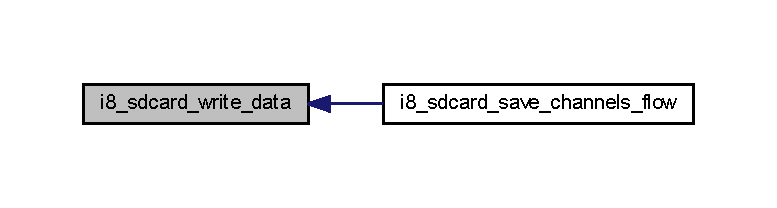
\includegraphics[width=350pt]{sd__manage__lib_8h_a9a526861ab82b18d6e3f4d46aac1579e_icgraph}
\end{center}
\end{figure}
\mbox{\Hypertarget{sd__manage__lib_8h_a81f7e2427d424cc9759559ba38f5b5e8}\label{sd__manage__lib_8h_a81f7e2427d424cc9759559ba38f5b5e8}} 
\index{sd\+\_\+manage\+\_\+lib.\+h@{sd\+\_\+manage\+\_\+lib.\+h}!i8\+\_\+sdcard\+\_\+write\+\_\+text@{i8\+\_\+sdcard\+\_\+write\+\_\+text}}
\index{i8\+\_\+sdcard\+\_\+write\+\_\+text@{i8\+\_\+sdcard\+\_\+write\+\_\+text}!sd\+\_\+manage\+\_\+lib.\+h@{sd\+\_\+manage\+\_\+lib.\+h}}
\subsubsection{\texorpdfstring{i8\+\_\+sdcard\+\_\+write\+\_\+text()}{i8\_sdcard\_write\_text()}}
{\footnotesize\ttfamily int8\+\_\+t i8\+\_\+sdcard\+\_\+write\+\_\+text (\begin{DoxyParamCaption}\item[{char $\ast$}]{filename,  }\item[{uint32\+\_\+t}]{u32\+\_\+addr,  }\item[{char $\ast$}]{c\+\_\+text }\end{DoxyParamCaption})}



Write a string data the given address in file. 


\begin{DoxyParams}[1]{Parameters}
\mbox{\tt in}  & {\em filename} & name of file \\
\hline
\mbox{\tt in}  & {\em u32\+\_\+addr} & address to write \\
\hline
\mbox{\tt in}  & {\em c\+\_\+text} & string write \\
\hline
\end{DoxyParams}
\begin{DoxyReturn}{Returns}
0\+: write success -\/1\+: file is not exist -\/2\+: can not write 
\end{DoxyReturn}
Here is the caller graph for this function\+:
\nopagebreak
\begin{figure}[H]
\begin{center}
\leavevmode
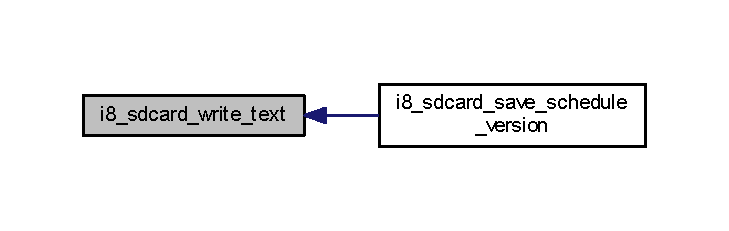
\includegraphics[width=350pt]{sd__manage__lib_8h_a81f7e2427d424cc9759559ba38f5b5e8_icgraph}
\end{center}
\end{figure}
\mbox{\Hypertarget{sd__manage__lib_8h_a132824b2516bca9a4c4994c4ec17ad54}\label{sd__manage__lib_8h_a132824b2516bca9a4c4994c4ec17ad54}} 
\index{sd\+\_\+manage\+\_\+lib.\+h@{sd\+\_\+manage\+\_\+lib.\+h}!i8\+\_\+sdcard\+\_\+write\+\_\+value@{i8\+\_\+sdcard\+\_\+write\+\_\+value}}
\index{i8\+\_\+sdcard\+\_\+write\+\_\+value@{i8\+\_\+sdcard\+\_\+write\+\_\+value}!sd\+\_\+manage\+\_\+lib.\+h@{sd\+\_\+manage\+\_\+lib.\+h}}
\subsubsection{\texorpdfstring{i8\+\_\+sdcard\+\_\+write\+\_\+value()}{i8\_sdcard\_write\_value()}}
{\footnotesize\ttfamily int8\+\_\+t i8\+\_\+sdcard\+\_\+write\+\_\+value (\begin{DoxyParamCaption}\item[{char $\ast$}]{filename,  }\item[{uint32\+\_\+t}]{u32\+\_\+addr,  }\item[{int32\+\_\+t}]{i32\+\_\+value }\end{DoxyParamCaption})}



Write a value to the given address in file. 


\begin{DoxyParams}[1]{Parameters}
\mbox{\tt in}  & {\em filename} & name of file \\
\hline
\mbox{\tt in}  & {\em u32\+\_\+addr} & address to write, the address must divisible by 4 \\
\hline
\mbox{\tt in}  & {\em i32\+\_\+value} & value to write \\
\hline
\end{DoxyParams}
\begin{DoxyReturn}{Returns}
0\+: write success -\/1\+: file is not exist -\/2\+: can not write 
\end{DoxyReturn}
$<$file is not exist Here is the caller graph for this function\+:
\nopagebreak
\begin{figure}[H]
\begin{center}
\leavevmode
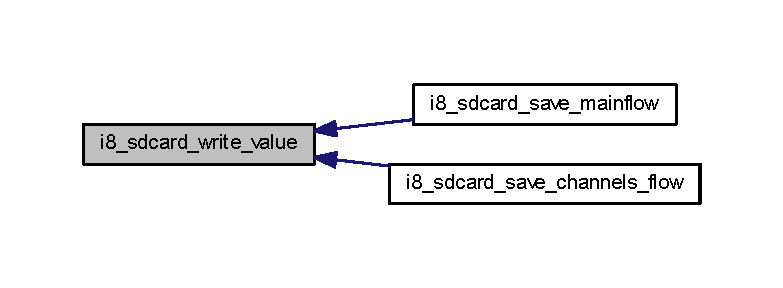
\includegraphics[width=350pt]{sd__manage__lib_8h_a132824b2516bca9a4c4994c4ec17ad54_icgraph}
\end{center}
\end{figure}

%--- End generated contents ---

% Index
\backmatter
\newpage
\phantomsection
\clearemptydoublepage
\addcontentsline{toc}{chapter}{Index}
\printindex

\end{document}
